\documentclass{cumcmthesis}

\usepackage[framemethod=TikZ]{mdframed}
\usepackage{url}
\usepackage{float}
\usepackage{array}
\usepackage{tabularx}
\usepackage{subcaption}

\graphicspath{{figures/}}

\newcommand{\kwh}{\mathrm{kWh}}
\newcommand{\yuan}{\text{元}}
\newcommand{\Tset}{\mathcal{T}}

\title{微网外部购电与储能调度优化研究}

\begin{document}

\maketitle

\begin{abstract}
\textbf{针对问题一：}将功率数据转换为十分钟电量，建立含供需平衡、储能效率、容量、功率和日循环约束的确定性线性规划。基准日结果显示，储能优化使购电费用由无储能方案的48052.05元降至35126.95元，下降26.90\%。

\textbf{针对问题二：}在每日0:00只使用前14天历史净负荷，采用经验均值和经验标准差构造安全净负荷，建立机会约束的日前模型，并用334天真实数据回测。固定安全系数$K=0.80$时，总成本为1654.76万元，紧急购电量为14.67万kWh。

\textbf{针对问题三：}对每天0:00、6:00、12:00和18:00发布的光伏预报进行跨日截断和线性插值，在计划偏差结算规则下建立MPC滚动模型。主方案$\alpha=0.95$的总成本为1368.87万元，相对仅执行0:00计划节省8.03\%。

\textbf{针对问题四：}将基础分时电价替换为按日期和时段变化的动态电价，分别重算机会约束日前模型和MPC模型。4-2与4-3总成本分别为1740.24万元和1433.19万元；在相同4-3模型下，MPC相对0:00固定计划节省121.14万元，节省率为7.79\%。

综上，实验表明储能跨时段转移、风险裕度和预测更新共同决定微网调度的经济性与供电可靠性；所有结论均限定在题目数据、日循环边界和本文回测口径内。

\keywords{微网调度\quad 储能优化\quad 机会约束\quad 模型预测控制\quad 动态电价}
\end{abstract}

\section{引言}

\subsection{问题背景}

微网由小区负荷、光伏发电、储能设备和外部电网构成。题目提供附件1至附件4，分别包含基础电价、全年负荷与实际光伏、四个时刻发布的光伏预测以及动态电价。每天划分为144个连续的十分钟时段，储能容量为12000\kwh，充放电功率上限为5000\kW，充放电效率均为0.9，2025年1月1日0:00的储电量为6000\kwh，并要求运行过程中储电量保持在1200至10800\kwh之间。

微网调度的关键在于同时处理时间耦合和信息不完全两类约束。储能可以把低价时段或光伏富余时段的电量转移到高价时段，但充放电效率、容量和功率上限会限制这种转移；另一方面，日前计划只能依据当时可获得的预测信息，实际负荷和光伏偏差会引发紧急购电或弃光。因此，单纯比较计划购电费用不足以评价策略，必须将计划、执行和事后结算放在同一条逻辑链上。

\subsection{问题重述}

四个问题具有清晰的递进关系：问题一假定全天负荷和光伏预测已知，求确定性日前计划；问题二只在每日0:00使用历史信息制定计划，并用实际数据评价紧急购电风险；问题三在新的光伏预测到达后滚动调整尚未执行的计划；问题四进一步考虑电价随日期和时段变化的情形，并分别完成机会约束日前优化和动态电价MPC调整。

\subsection{总体分析}

本文按“基准模型--风险模型--反馈模型--价格扩展”的顺序推进。先在已知预测下求解问题一，验证储能设备是否能够通过跨时段转移降低费用；再把问题一推广至全年，并在问题二中用历史净负荷统计量构造日前安全裕度；随后在问题三中引入四个时刻的光伏预报，建立预测更新和储能状态反馈闭环；最后在问题四中将基础电价替换为日期--时段动态电价，检验风险控制与峰谷套利的共同作用。

本文坚持三个实验原则。第一，所有决策变量统一使用十分钟电量，避免在目标函数、能量平衡和储能递推中混用功率与电量。第二，严格区分决策时可获得的信息和事后评价使用的真实数据，避免以真实数据构成“完美预测”。第三，每项实验都对应明确的验证问题：无储能对照验证经济收益，$K$扫描验证风险--成本权衡，MPC固定计划对照验证滚动更新的边际收益，$\alpha$和$\beta$敏感性验证参数选择的稳健性。

\section{模型假设与符号说明}

\subsection{模型假设}

为突出购电计划和储能调度的主要矛盾，作如下假设：
\begin{enumerate}
    \item 所有功率数据在十分钟时段内按常值处理，功率与电量通过式（2）换算；
    \item 光伏优先供给本地负荷，不能被负荷或储能吸收的富余光伏不向外网反送，计为弃光；
    \item 储能充放电效率恒定为0.9，且不设置同一时段同时充放电的额外二进制变量；正电价和效率损耗下，线性规划最优解通常不会主动安排这种无效循环；
    \item 问题二和4-2的净负荷统计仅使用目标日之前14天的历史样本；问题三和4-3的滚动优化仅使用对应发布时间已经获得的预测；
    \item 问题三沿用问题二的紧急购电5倍电价口径，以便三层费用可以在同一回测框架内比较；
    \item 每日采用始末储电量均为6000 kWh的闭环边界，因而回测结果用于逐日比较，不代表全年连续运行状态。
\end{enumerate}

\subsection{数据预处理与统一量纲}

记日内时段集合为$\Tset=\{0,1,\ldots,143\}$，单个时段长度为
\begin{equation}
    \Delta t=\frac{10}{60}=\frac{1}{6}\ \mathrm{h}.
    \tag{1}
\end{equation}
若输入的负荷功率和光伏功率分别为$P_{\mathrm{load},d,t}$和$P_{\mathrm{pv},d,t}$，则对应的时段电量为
\begin{equation}
    E_{\mathrm{load},d,t}=P_{\mathrm{load},d,t}\Delta t,qquad
    E_{\mathrm{pv},d,t}=P_{\mathrm{pv},d,t}\Delta t.
    \tag{2}
\end{equation}
定义实际净负荷为
\begin{equation}
    N_{d,t}=E_{\mathrm{load},d,t}-E_{\mathrm{pv},d,t}.
    \tag{3}
\end{equation}

\subsection{统一设备约束}

记$E_{\mathrm{ch},d,t}$和$E_{\mathrm{dis},d,t}$为储能充电量和放电量，$S_{d,t}$为时段边界处的储电量。储能状态满足
\begin{equation}
S_{d,t+1}=S_{d,t}+\eta_{\mathrm{ch}}E_{\mathrm{ch},d,t}
-\frac{E_{\mathrm{dis},d,t}}{\eta_{\mathrm{dis}}},
\qquad \eta_{\mathrm{ch}}=\eta_{\mathrm{dis}}=0.9.
\tag{4}
\end{equation}
单个十分钟时段的充放电上限为
\begin{equation}
0\leq E_{\mathrm{ch},d,t},E_{\mathrm{dis},d,t}
\leq E_{\max}=5000\Delta t=833.3333\ \kwh,
\tag{5}
\end{equation}
并满足
\begin{equation}
1200\leq S_{d,t}\leq10800,\qquad S_{d,0}=S_{d,144}=6000.
\tag{6}
\end{equation}
本文不考虑向外部电网反向售电，因此所有普通购电量均非负。

\begin{table}[H]
\centering
\renewcommand\arraystretch{1.2}
\caption{统一符号说明}
\label{tab:symbols}
\begin{tabular}{p{3.5cm}p{7.3cm}p{2.0cm}}
\toprule
\textbf{符号} & \textbf{含义} & \textbf{单位}\\
\midrule
$d,t$ & 日期和十分钟时段索引 & --\\
$C_{d,t}$、$p_t$ & 动态电价和基础分时电价 & 元/kWh\\
$E_{\mathrm{grid},d,t}$ & 外部电网普通购电量 & kWh\\
$E^0_{d,t}$、$E_{d,t}$ & 0:00原始计划和滚动调整后的购电量 & kWh\\
$E_{\mathrm{load},d,t}$、$E_{\mathrm{pv},d,t}$ & 负荷电量和实际光伏电量 & kWh\\
$\widehat E^{(r)}_{\mathrm{pv},d,t}$ & 发布时刻$r$形成的光伏预测电量 & kWh\\
$E_{\mathrm{emer},d,t}$、$E_{\mathrm{curt},d,t}$ & 紧急购电量和弃光量 & kWh\\
$u^+_{d,t}$、$u^-_{d,t}$ & 增购量和退订量辅助变量 & kWh\\
$K$、$\alpha$、$\beta$ & 安全裕度、预测折减和动态电价场景折减系数 & --\\
\bottomrule
\end{tabular}
\end{table}

\subsection{实验数据与评价口径}

问题一使用题目指定的单日数据。问题二至问题四均以2025年2月1日至12月31日为回测区间，共334天；问题二和问题四的日前统计量使用前14天历史净负荷，但问题二采用分母为$W$的经验标准差，4-2采用分母为$W-1$的无偏标准差。每日优化均采用$S_{d,0}=S_{d,144}=6000$的日循环边界，因此各日结果可独立比较，但不能直接解释为全年连续运行的储能轨迹。

\section{实验设计与评价指标}

本文将实验视为模型论证的一部分，而不是求解后的附加展示。对每个方案，先根据该方案在决策时可获得的信息求解线性规划，再把生成的购电和储能轨迹输入真实负荷、实际光伏和相应电价，最后进行统一结算。这样得到的总成本由普通购电、计划偏差和紧急购电三类费用构成；弃光量不直接计入费用，但作为可再生能源消纳指标单独统计。

对问题一，使用无储能方案作为经济性基准，并检查储能容量和始末状态约束。对问题二，先进行固定$K$粗扫，再在低成本区间细扫，观察总成本、紧急购电和弃光量的变化。对问题三，在相同的0:00计划基准下比较不同$\alpha$的MPC方案，并分析预测发布时间与紧急购电的关系。对问题四，分别比较4-2与4-3的综合表现，以及4-3中MPC与0:00固定计划的边际差异；同时对$K$和$\beta$进行单因素敏感性分析。

\begin{table}[H]
\centering
\scriptsize
\renewcommand\arraystretch{1.25}
\caption{四个问题的决策信息、模型和实验目的}
\label{tab:research_design}
\begin{tabularx}{\textwidth}{p{1.2cm}p{3.1cm}p{3.3cm}X}
\toprule
\textbf{问题} & \textbf{决策时信息} & \textbf{核心模型} & \textbf{实验目的}\\
\midrule
1 & 单日已知电价、负荷和光伏预测 & 确定性线性规划 & 以无储能方案为基准，验证储能套利和物理可行性\\
2 & 0:00可用前14天历史数据 & 机会约束日前规划 & 通过$K$扫描识别普通购电与紧急购电之间的权衡\\
3 & 0:00、6:00、12:00、18:00的光伏预报 & MPC滚动线性规划 & 以固定0:00计划为基准，验证预测更新的边际收益\\
4 & 问题二、三的信息加动态电价 & 动态电价机会约束与MPC & 分离动态价格影响和滚动修正影响，并检验$K,\beta$敏感性\\
\bottomrule
\end{tabularx}
\end{table}

定义回测期内的总成本、紧急购电天数、紧急购电量和弃光量为
\begin{equation}
\begin{aligned}
Z&=\sum_d(C_{\mathrm{buy},d}+C_{\mathrm{dev},d}+C_{\mathrm{emer},d}),\\
D_{\mathrm{emer}}&=\sum_d\mathbf{1}\left(\sum_tE_{\mathrm{emer},d,t}>10^{-4}\right),\\
Q_{\mathrm{emer}}&=\sum_{d,t}E_{\mathrm{emer},d,t},\qquad
Q_{\mathrm{curt}}=\sum_{d,t}E_{\mathrm{curt},d,t}.
\end{aligned}
\tag{7a}
\end{equation}
其中，$C_{\mathrm{dev},d}$在问题一、问题二和4-2中为零；问题三和4-3按照题目偏差规则结算。比较策略时，以总成本作为经济性主指标，以$Q_{\mathrm{emer}}$和$D_{\mathrm{emer}}$描述供电风险，以$Q_{\mathrm{curt}}$描述光伏消纳损失。

\section{问题一：确定性日前购电与储能优化}

\subsection{模型建立}

在全天负荷、光伏预测和电价均已知时，令$E_{\mathrm{grid},t}$为购电量，建立确定性线性规划：
\begin{equation}
\min Z_1=\sum_{t\in\Tset}p_tE_{\mathrm{grid},t}.
\tag{7}
\end{equation}
供需平衡为
\begin{equation}
E_{\mathrm{grid},t}+E_{\mathrm{pv},t}+E_{\mathrm{dis},t}
\geq E_{\mathrm{load},t}+E_{\mathrm{ch},t},\qquad t\in\Tset.
\tag{8}
\end{equation}
式（4）至式（6）构成储能的状态、容量、功率和日循环约束。模型的物理含义是：光伏和外部电网共同满足负荷，储能可以在低价时段充电、在高价时段放电，但不能突破设备边界。

\subsection{求解结果与合理性检验}

采用HiGHS线性规划求解器得到基准日最优解。结果如表~\ref{tab:q1result}所示。全天购电量为59482.70\kwh，购电费用为35126.95元；储能累计充电20740.67\kwh、放电16799.94\kwh，终止储电量为6000\kwh。

\begin{table}[H]
\centering
\renewcommand\arraystretch{1.2}
\caption{问题一基准日优化结果}
\label{tab:q1result}
\begin{tabular}{lrr}
\toprule
\textbf{指标} & \textbf{优化结果} & \textbf{说明}\\
\midrule
全天购电量 & 59482.70 kWh & 普通购电\\
全天购电费用 & 35126.95 元 & 目标函数值\\
累计充电量 & 20740.67 kWh & 计入充电效率前\\
累计放电量 & 16799.94 kWh & 储能输出侧电量\\
始末储电量 & 6000 / 6000 kWh & 满足日循环\\
\bottomrule
\end{tabular}
\end{table}

如图~\ref{fig:q1dispatch}所示，最优解在低价时段安排充电，在高价时段安排放电；中午光伏出力较高时，储能还能够吸收部分富余光伏。图~\ref{fig:q1soc}显示储电量始终处于1200至10800\kwh范围内，且首尾相接。与“光伏优先、无储能”的基准方案相比，购电费用减少
\begin{equation}
48052.05-35126.95=12925.10\ \text{元},
\tag{9}
\end{equation}
降幅为26.90\%，说明模型同时具有物理可行性和经济合理性。

\begin{figure}[H]
\centering
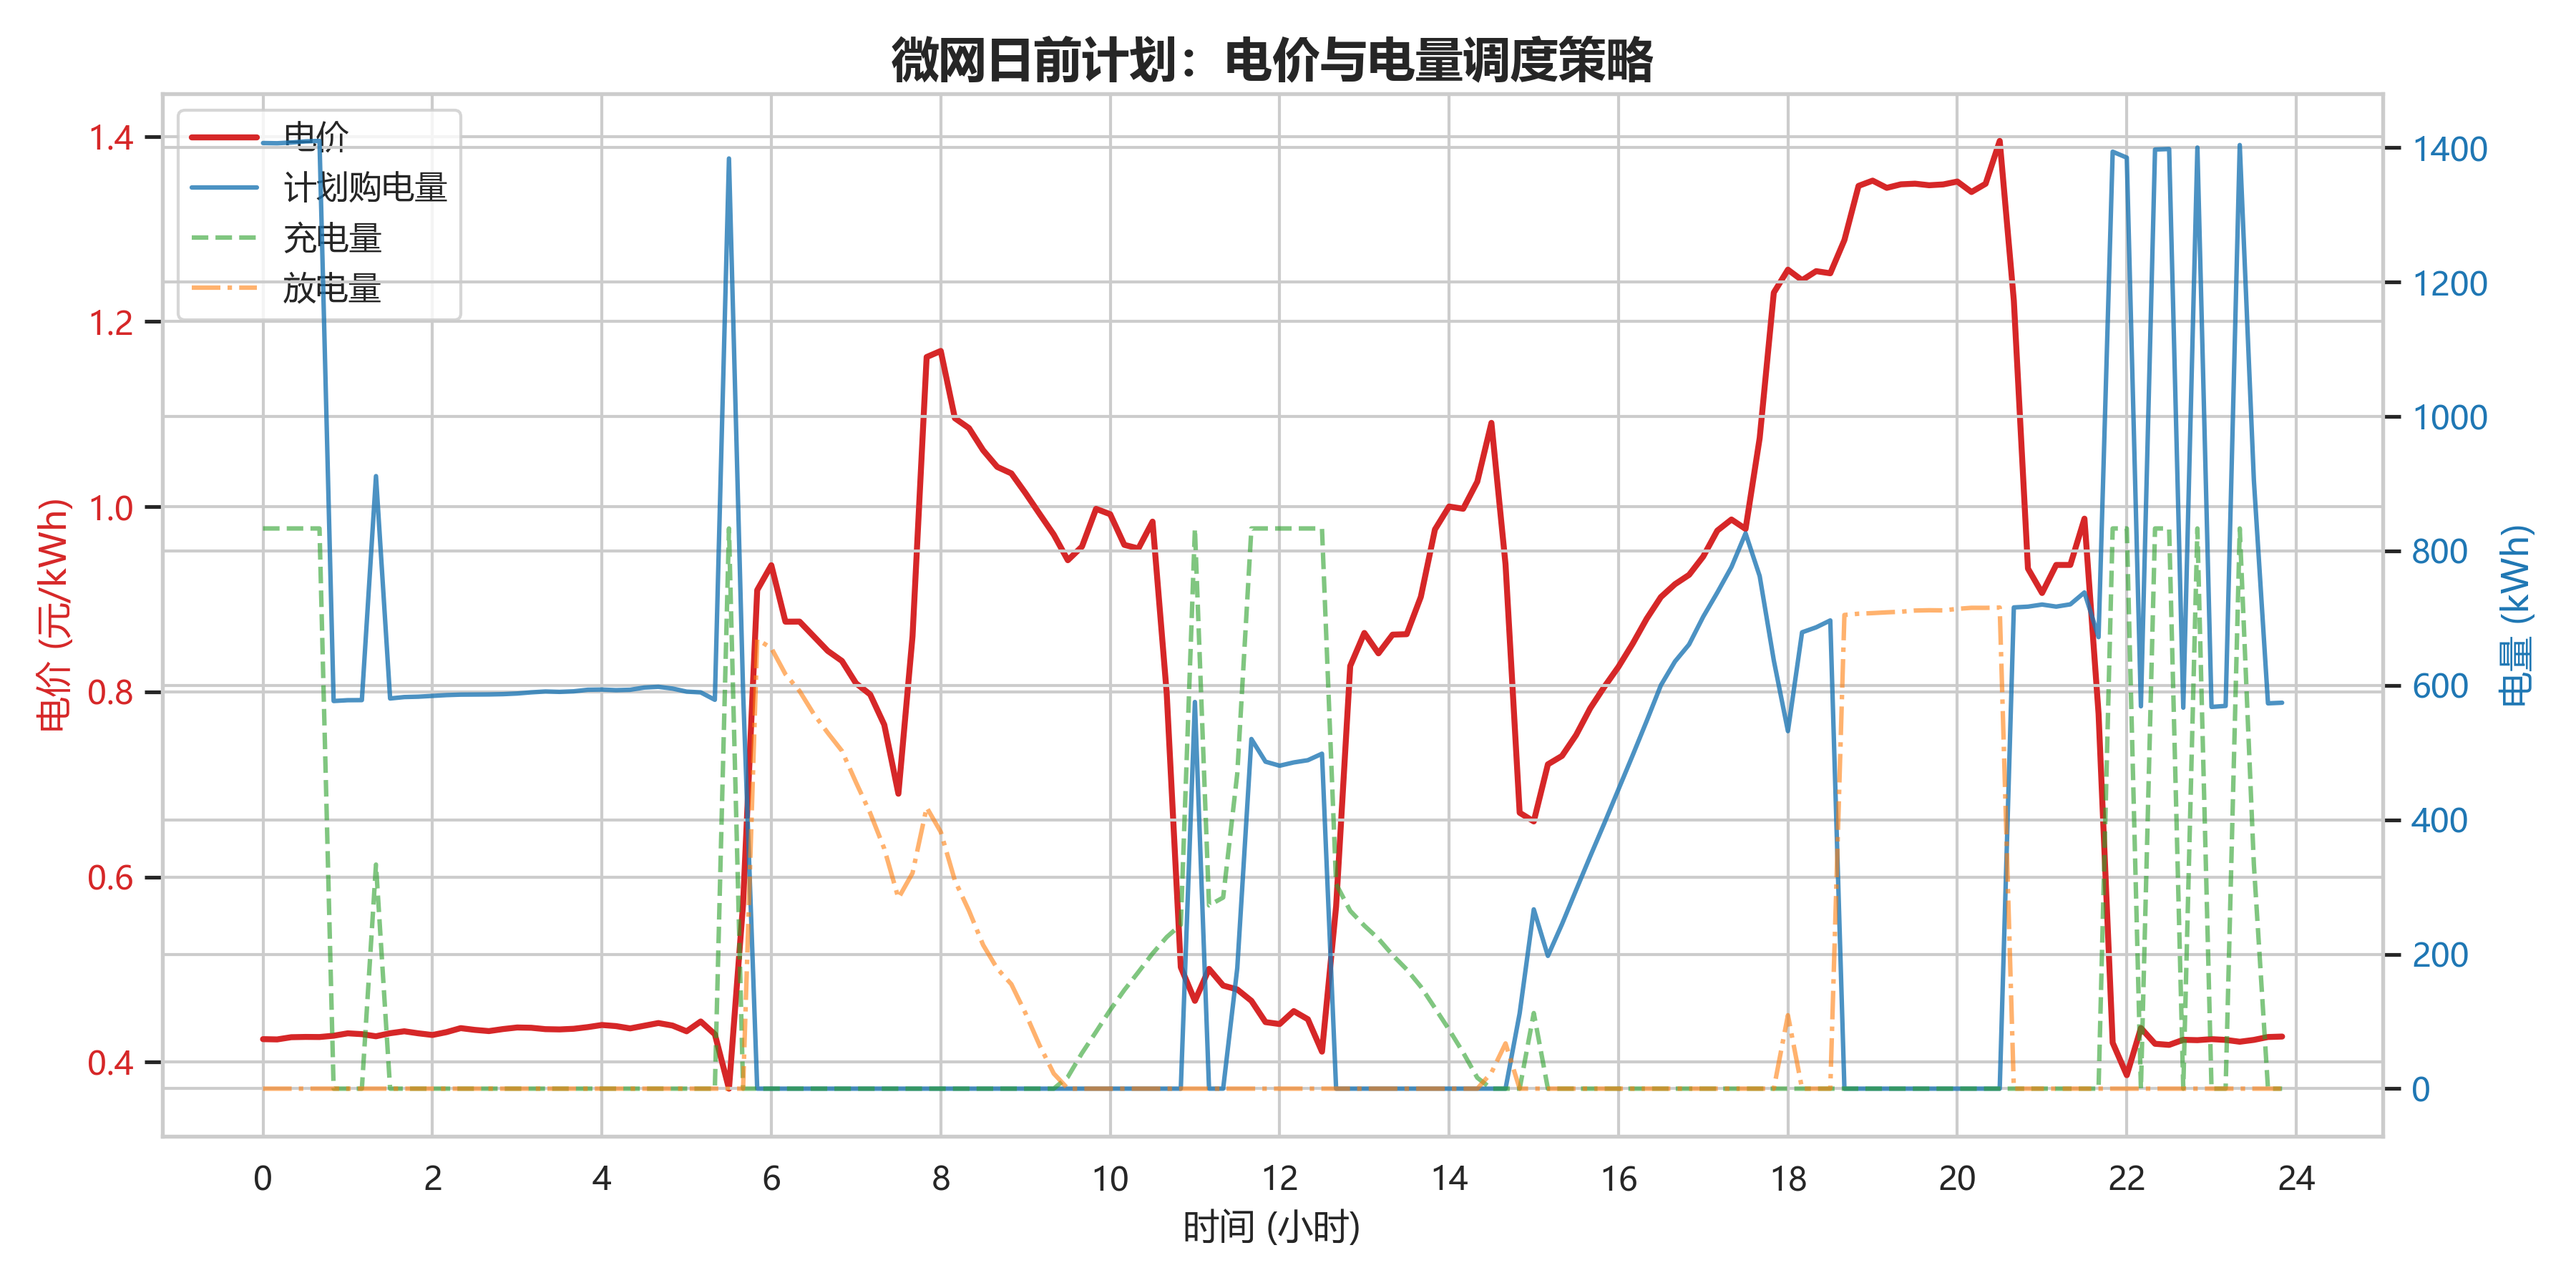
\includegraphics[width=.86\textwidth]{q1_dispatch.png}
\caption{问题一电价与购电、储能调度}
\label{fig:q1dispatch}
\end{figure}

\begin{figure}[H]
\centering
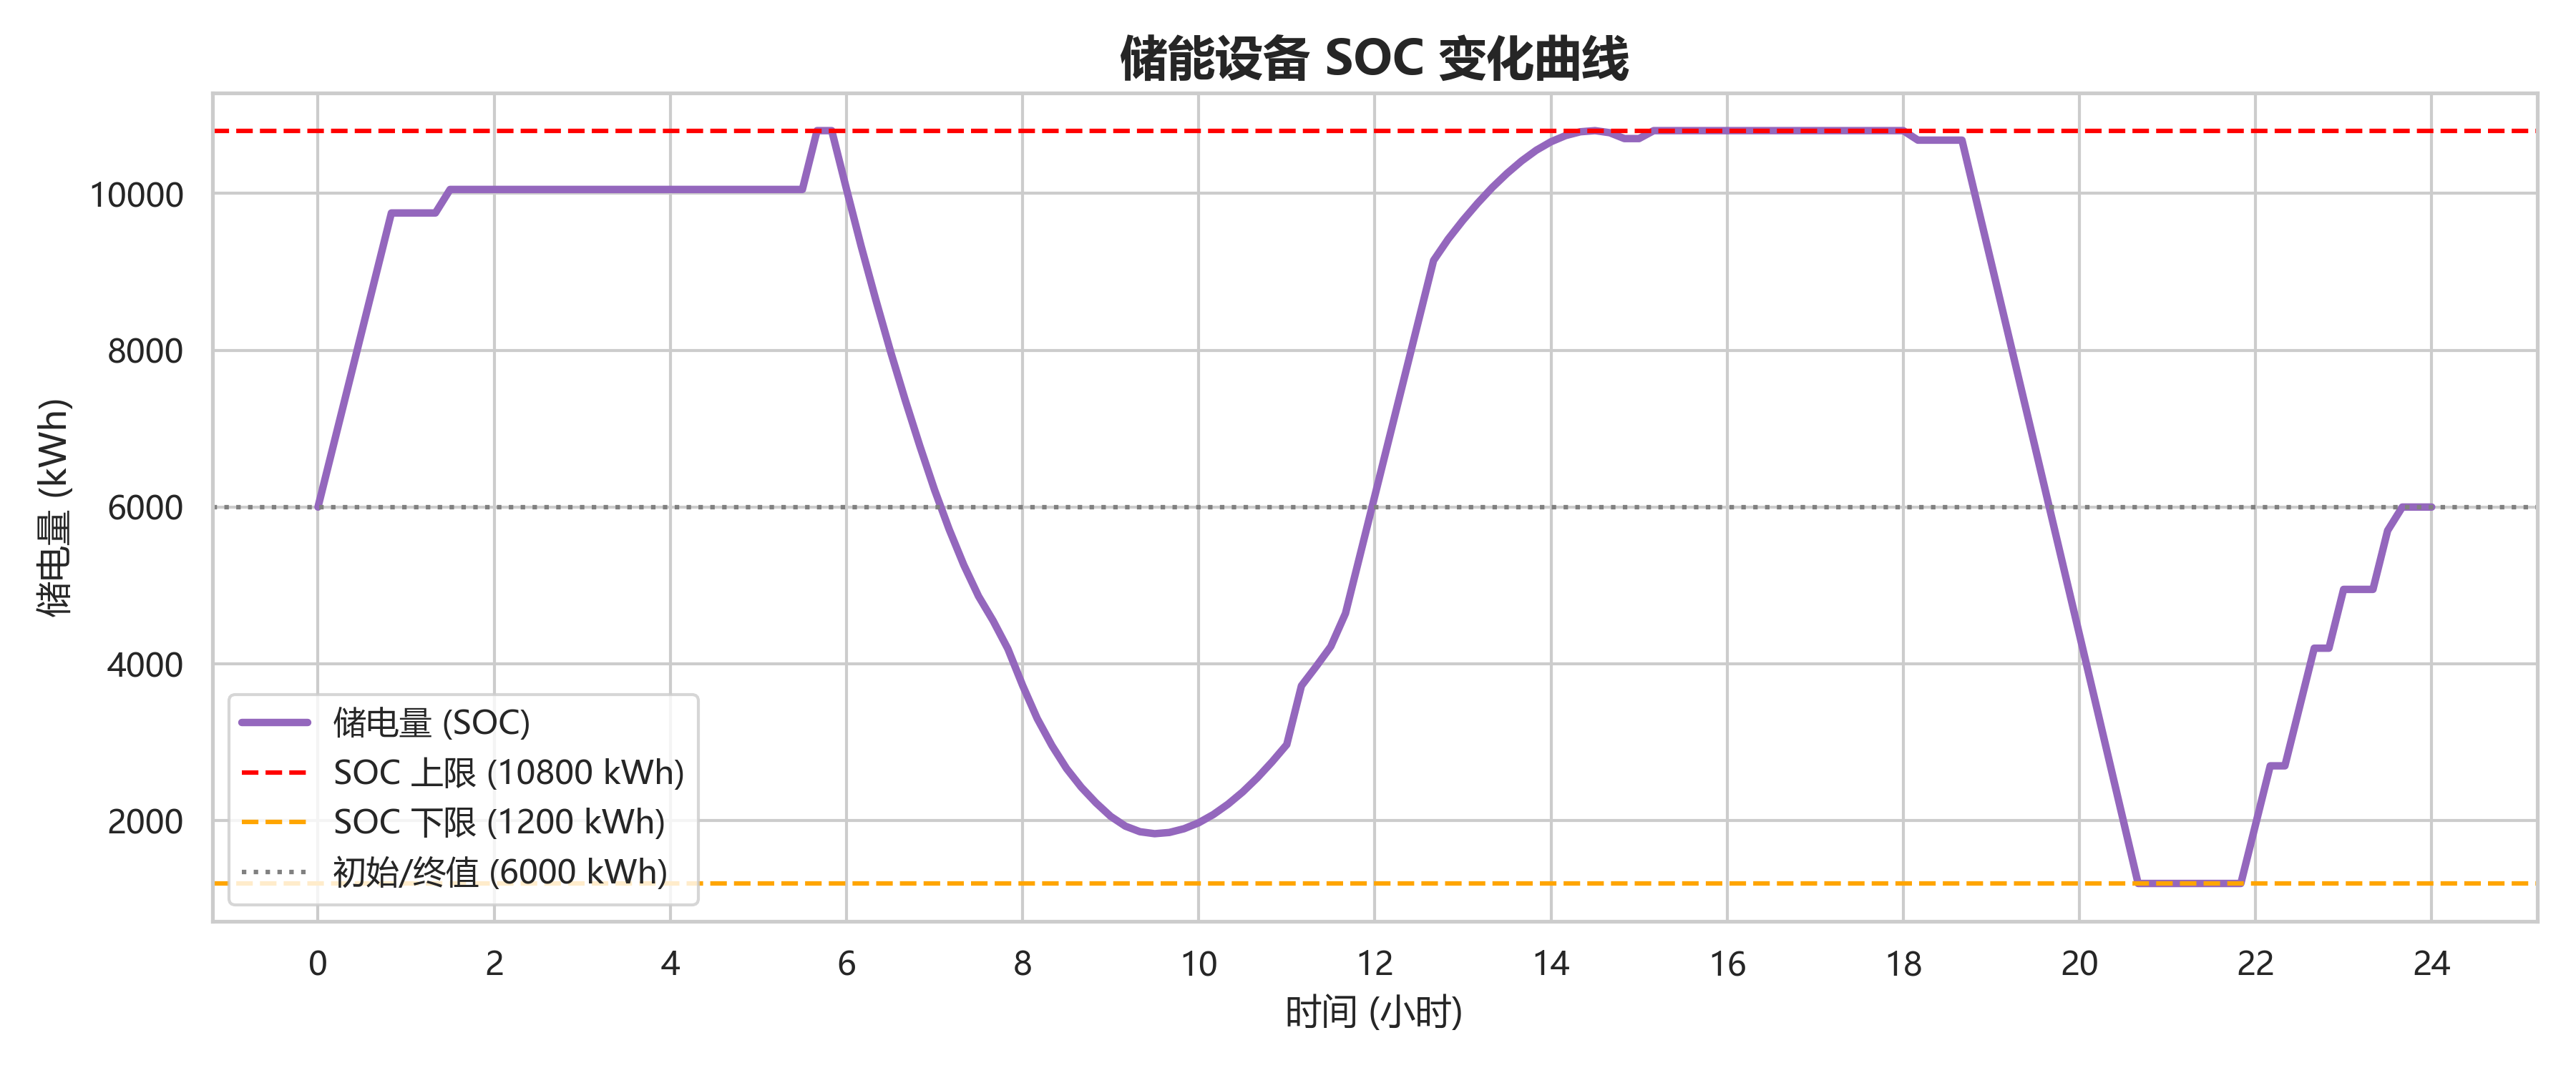
\includegraphics[width=.86\textwidth]{q1_soc.png}
\caption{问题一储能储电量变化}
\label{fig:q1soc}
\end{figure}

\section{问题二：机会约束日前优化与真实回测}

\subsection{历史统计与机会约束确定性等价}

问题二在每天0:00制定全天计划，决策时不能使用当天真实负荷和光伏。对日期$d$，用前$W=14$天同一时段的净负荷样本计算
\begin{equation}
\mu_{d,t}=\frac{1}{W}\sum_{j=d-W}^{d-1}N_{j,t},\qquad
\sigma_{d,t}=\sqrt{\frac{1}{W}\sum_{j=d-W}^{d-1}(N_{j,t}-\mu_{d,t})^2}.
\tag{10}
\end{equation}
这里采用程序中的经验标准差（分母为$W$）；问题四4-2的程序则采用无偏标准差（分母为$W-1$），两者的计算口径分别保持与对应结果文件一致。
在净负荷近似服从正态分布的条件下，对供电能力设置机会约束
\begin{equation}
\mathbb P\left(E^0_{d,t}+E_{\mathrm{dis},d,t}-E_{\mathrm{ch},d,t}\geq N_{d,t}\right)\geq1-\alpha
\tag{11}
\end{equation}
可转化为
\begin{equation}
E^0_{d,t}+E_{\mathrm{dis},d,t}-E_{\mathrm{ch},d,t}
\geq\mu_{d,t}+K\sigma_{d,t},qquad K=\Phi^{-1}(1-\alpha).
\tag{12}
\end{equation}
这里的$K$是可解释的安全裕度系数，但式（12）只表示逐时段正态近似，并不保证全天144个时段的联合覆盖率。

\subsection{日前计划和日内评估}

日前线性规划目标为
\begin{equation}
\min Z_{2,\mathrm{DA}}=\sum_{t\in\Tset}p_tE^0_{d,t},
\tag{13}
\end{equation}
并结合式（4）至式（6）及式（12）。计划确定后，用当天真实数据计算实际盈余
\begin{equation}
R_{d,t}=E_{\mathrm{pv},d,t}+E^0_{d,t}+E_{\mathrm{dis},d,t}
-E_{\mathrm{ch},d,t}-E_{\mathrm{load},d,t}.
\tag{14}
\end{equation}
若$R_{d,t}<0$，紧急购电量为$E_{\mathrm{emer},d,t}=\max(0,-R_{d,t})$；若$R_{d,t}>0$，将富余部分记为弃光量$E_{\mathrm{curt},d,t}=\max(0,R_{d,t})$。最终回测成本为
\begin{equation}
Z_2=\sum_{d,t}p_tE^0_{d,t}+5\sum_{d,t}p_tE_{\mathrm{emer},d,t}.
\tag{15}
\end{equation}
这一区分保证日前模型没有偷用当天真实数据，而风险指标仍然由真实运行结果检验。

\subsection{参数扫描与结果}

对$K=0.40,0.50,\ldots,2.00$进行粗扫，并在$0.80$至$0.85$区间以0.01为步长细扫。粗扫呈现先降后升的谷形：$K$过小时普通购电费用低但紧急购电罚费高；$K$过大时紧急购电下降，但普通购电和弃光增加。细扫中$K=0.81$仅比$K=0.80$低约0.08万元，差异不足总成本的0.01\%，因此采用参数更简洁、便于实施的$K=0.80$。

\begin{table}[H]
\centering
\scriptsize
\renewcommand\arraystretch{1.2}
\caption{问题二安全裕度敏感性摘要}
\label{tab:q2scan}
\begin{tabular}{ccrrr}
\toprule
$K$ & 总成本（万元） & 紧急天数 & 紧急购电（万kWh） & 弃光（万kWh）\\
\midrule
0.40 & 2058.18 & 233 & 112.87 & 380.15\\
0.60 & 1756.70 & 222 & 47.75 & 454.89\\
0.80 & \textbf{1654.76} & 122 & 14.67 & 560.70\\
0.85 & 1657.69 & 102 & 10.83 & 591.20\\
1.00 & 1699.22 & 63 & 4.32 & 688.89\\
1.30 & 1845.65 & 19 & 0.86 & 896.28\\
1.80 & 2128.62 & 1 & 0.00 & 1245.92\\
2.00 & 2245.78 & 0 & 0.00 & 1385.86\\
\bottomrule
\end{tabular}
\end{table}

固定$K=0.80$的334天回测结果为：日前购电费1564.61万元，紧急购电罚费90.15万元，总成本1654.76万元，紧急购电122天、14.67万kWh，弃光560.70万kWh。动态安全裕度对照实验显示，基于历史光伏均值的简单分时规则虽然可以降低部分弃光，但可能在阴天造成欠购电，最终总成本高于固定$K=0.80$；因此不将其作为主方案。

\begin{figure}[H]
\centering
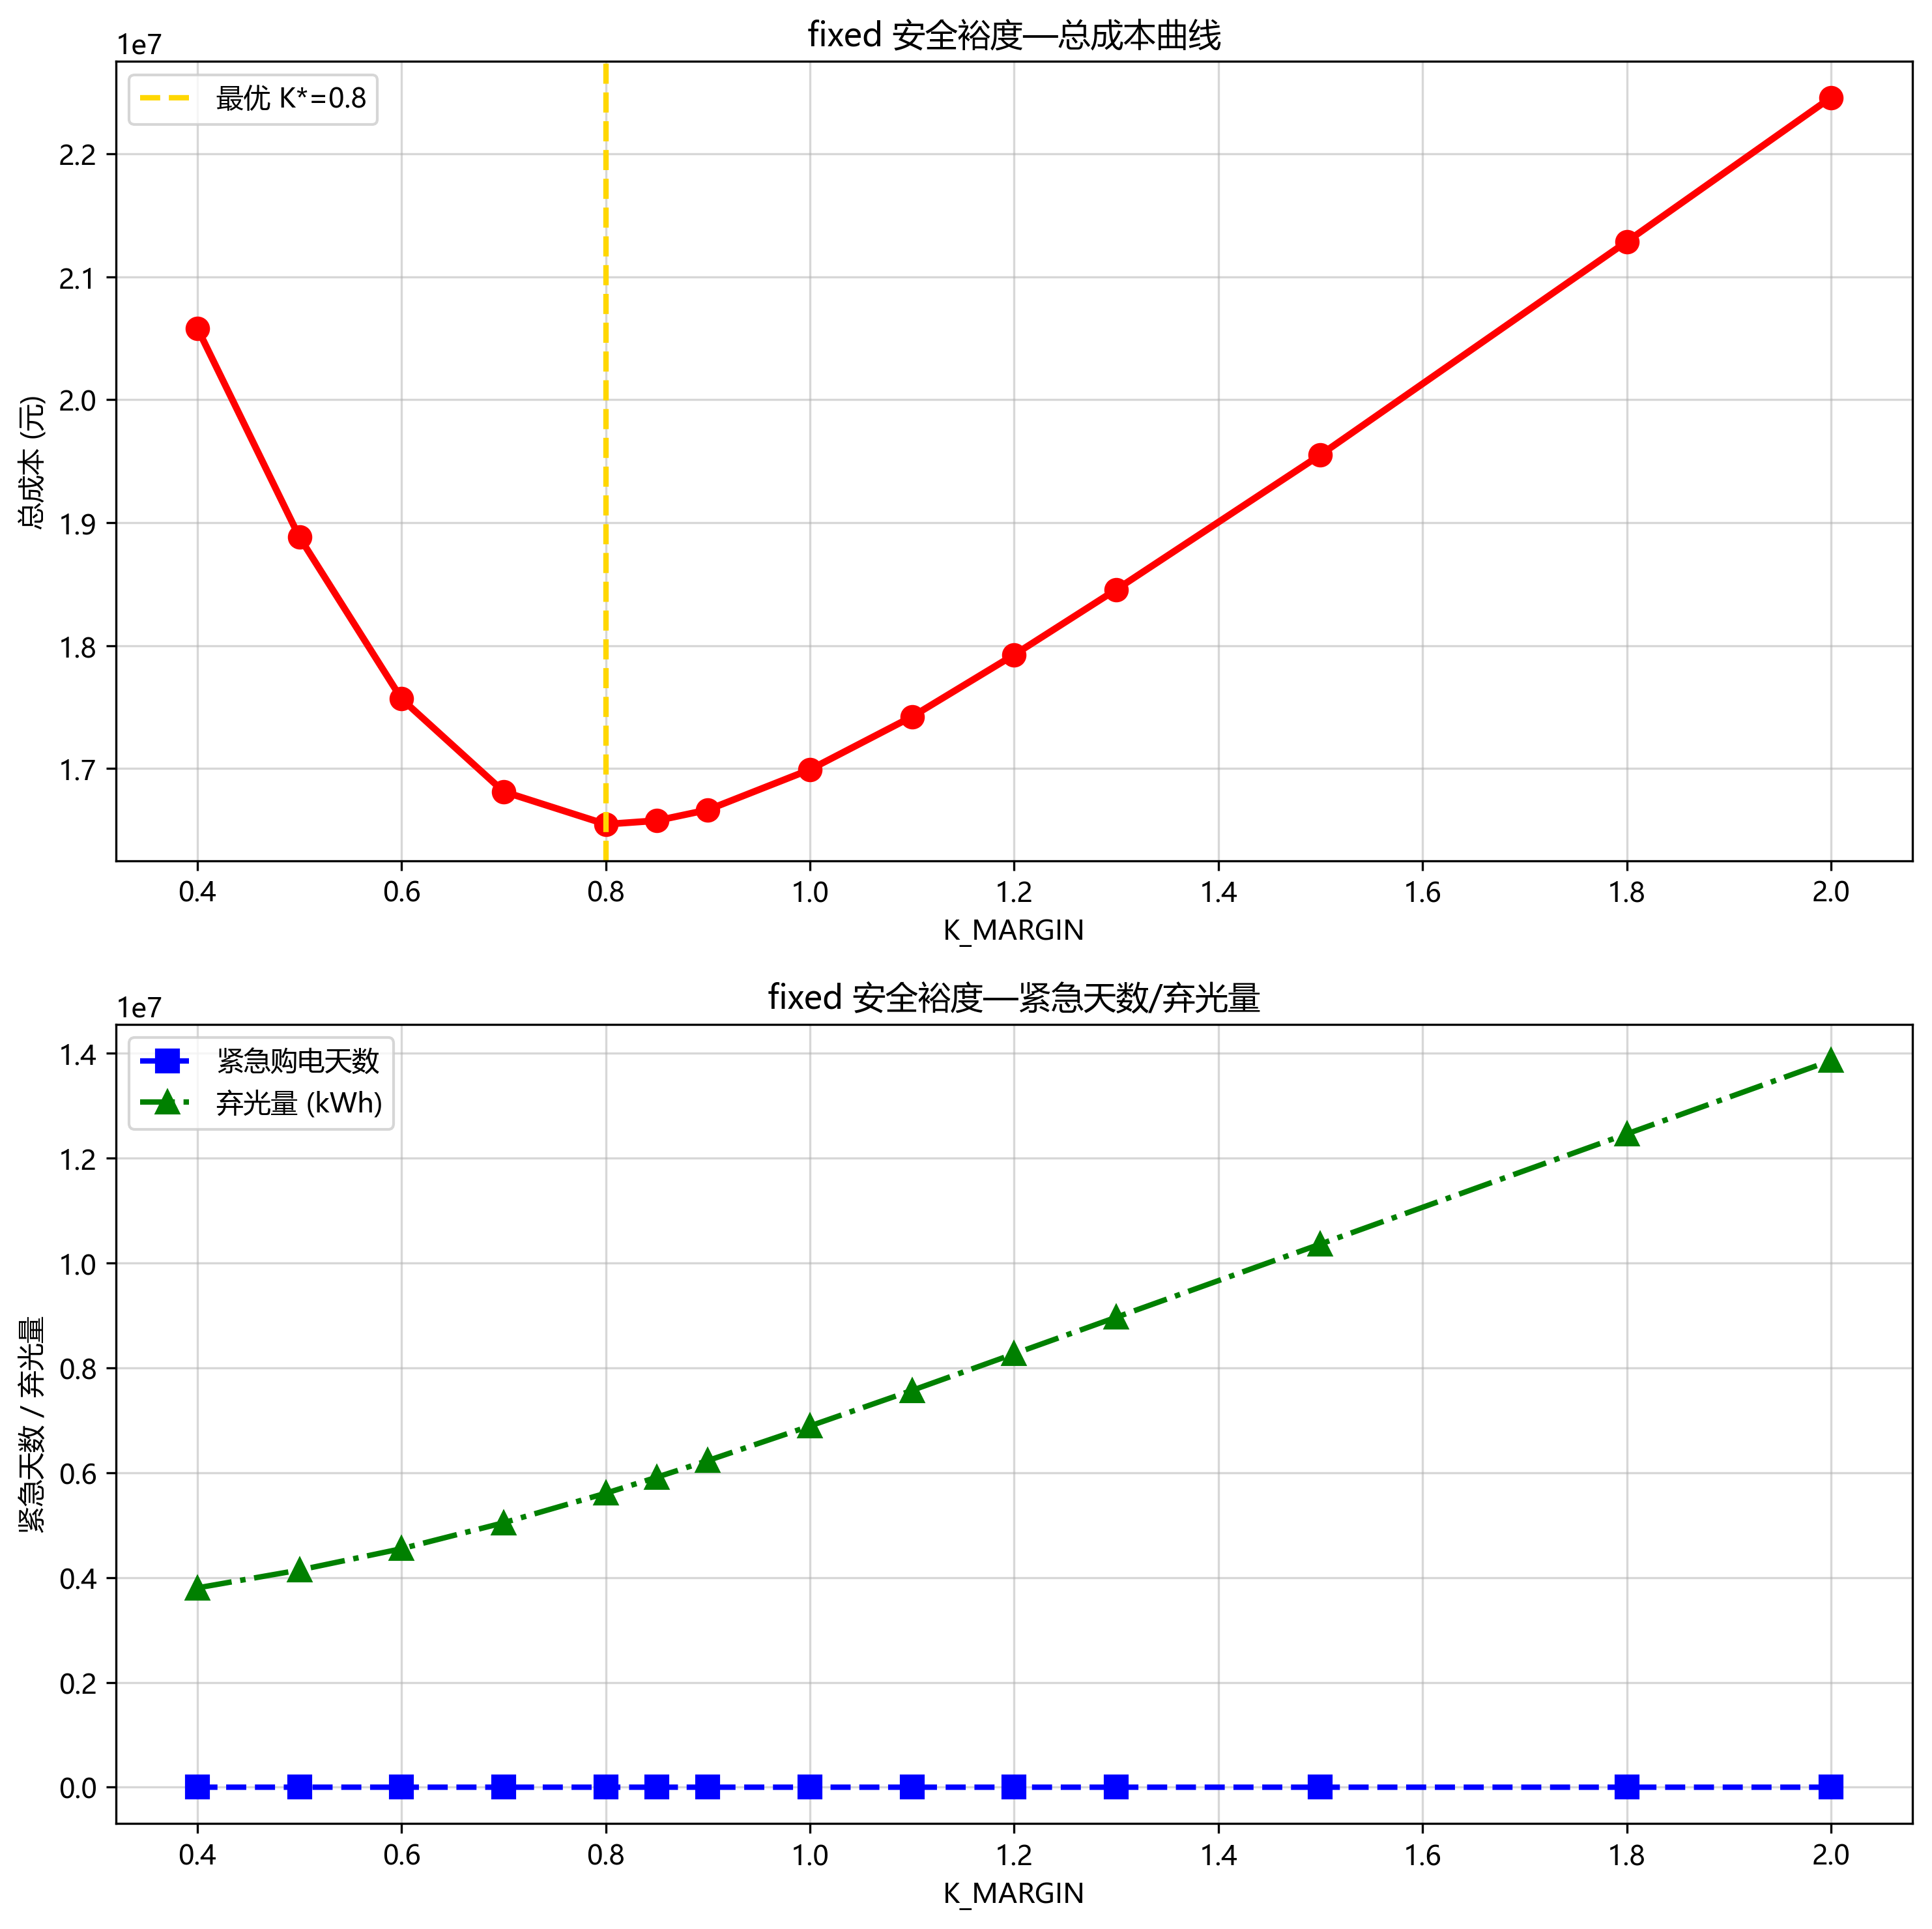
\includegraphics[width=.82\textwidth]{q2_k_scan.png}
\caption{问题二固定安全裕度粗扫}
\label{fig:q2scan}
\end{figure}

\section{问题三：光伏预测更新下的MPC滚动调度}

\subsection{预测序列构造}

附件3在每天0:00、6:00、12:00和18:00给出未来24小时的整点光伏预测。读取后先对日期列向前填充，再按发布时间分组。6:00预报只取当天7:00至24:00，12:00预报只取当天13:00至24:00，18:00预报只取当天19:00至24:00，跨日部分不进入当天剩余时域。对整点序列进行分段线性插值，得到十分钟预测；日内预测再乘以保守折减系数$\alpha$：
\begin{equation}
\widetilde E_{\mathrm{pv},d,t}^{(r)}=\alpha\widehat E_{\mathrm{pv},d,t}^{(r)},qquad r\in\{6,12,18\}.
\tag{16}
\end{equation}
主方案取$\alpha=0.95$。$\alpha$越小，预测越保守，通常会降低紧急购电，却可能增加常规购电和偏差成本。

\subsection{日前计划、滚动调整与执行轨迹}

0:00使用全天预测求解
\begin{equation}
\min Z_{3,0}=\sum_{t\in\Tset}p_tE^0_{d,t},qquad
E^0_{d,t}+E_{\mathrm{dis},d,t}-E_{\mathrm{ch},d,t}
\geq E_{\mathrm{load},d,t}-\widehat E^{(0)}_{\mathrm{pv},d,t}.
\tag{17}
\end{equation}
在更新断面$\tau\in\{35,71,107\}$，锁定已执行时段，以当前运行状态$S_{d,\tau}^{\mathrm{real}}$为初值，对剩余时域再优化。令$E_{d,t}$为调整后购电量，引入
\begin{equation}
E_{d,t}-E^0_{d,t}=u^+_{d,t}-u^-_{d,t},qquad u^+_{d,t},u^-_{d,t}\geq0.
\tag{18}
\end{equation}
根据题意，超计划购电按1.5倍电价，少购部分按原计划电价的50\%收取偏差费用。因此每一阶段的目标可写为
\begin{equation}
\min Z_{3,\tau}=\sum_{t=\tau}^{143}p_t
\left(E_{d,t}+0.5u^+_{d,t}+0.5u^-_{d,t}\right),
\tag{19}
\end{equation}
约束为
\begin{equation}
E_{d,t}+E_{\mathrm{dis},d,t}-E_{\mathrm{ch},d,t}
\geq E_{\mathrm{load},d,t}-\widetilde E_{\mathrm{pv},d,t}^{(\tau)}.
\tag{20}
\end{equation}
每次求解只执行下一个更新区间，全天购电和储能轨迹按
\begin{equation}
E^{\mathrm{exec}}=\left[E^0_{0:35},E^6_{35:71},E^{12}_{71:107},E^{18}_{107:144}\right]
\tag{21}
\end{equation}
拼接。真实回测使用附件2的实际负荷和实际光伏，紧急购电量为
\begin{equation}
E_{\mathrm{emer},d,t}=\max\left\{0,E_{\mathrm{load},d,t}-E_{\mathrm{pv},d,t}
-E^{\mathrm{exec}}_{d,t}-E^{\mathrm{exec}}_{\mathrm{dis},d,t}
+E^{\mathrm{exec}}_{\mathrm{ch},d,t}\right\}.
\tag{22}
\end{equation}

问题三原文只明确给出计划偏差结算规则，本文沿用问题二的“紧急购电按交易时刻电价5倍”口径，以便在同一回测体系下评价风险。日总成本由常规购电、偏差费用和紧急购电费用构成：
\begin{equation}
C_{3,d}=\sum_t p_tE^{\mathrm{exec}}_{d,t}
+0.5\sum_t p_t|E^{\mathrm{exec}}_{d,t}-E^0_{d,t}|
+5\sum_t p_tE_{\mathrm{emer},d,t}.
\tag{23}
\end{equation}

\subsection{回测结果与误差解释}

\begin{table}[H]
\centering
\renewcommand\arraystretch{1.2}
\caption{问题三滚动策略回测结果}
\label{tab:q3result}
\begin{tabular}{lrrr}
\toprule
\textbf{策略} & 总成本（万元） & 紧急购电（万kWh） & 节省比例\\
\midrule
仅执行0:00计划 & 1488.33 & 62.3295 & --\\
MPC，$\alpha=1.00$ & 1403.07 & 34.6951 & 5.73\%\\
MPC，$\alpha=0.98$ & 1376.30 & 23.7359 & 7.53\%\\
MPC，$\alpha=0.95$ & \textbf{1368.87} & 14.3596 & \textbf{8.03\%}\\
MPC，$\alpha=0.90$ & 1409.64 & 8.9414 & 5.29\%\\
\bottomrule
\end{tabular}
\end{table}

主方案$\alpha=0.95$的成本结构为：实际购电1275.68万元、偏差费用35.90万元、紧急购电费用57.29万元。与静态0:00计划相比，MPC同时降低综合成本和紧急购电量；继续降低$\alpha$虽可进一步减少紧急购电，但因保守购电和偏差增加而使总成本回升。334天预测误差统计中，0:00、6:00、12:00和18:00预测的平均绝对误差分别为207.47、176.44、88.79和7.20 kW，说明新预测的到达确实提供了有价值的信息。紧急购电主要集中在清晨光伏爬坡和傍晚光伏下降阶段；6:00预测误差与当日紧急购电量的Pearson相关系数为0.660，但该相关关系仅作风险解释，不构成因果识别。

\begin{figure}[H]
\centering
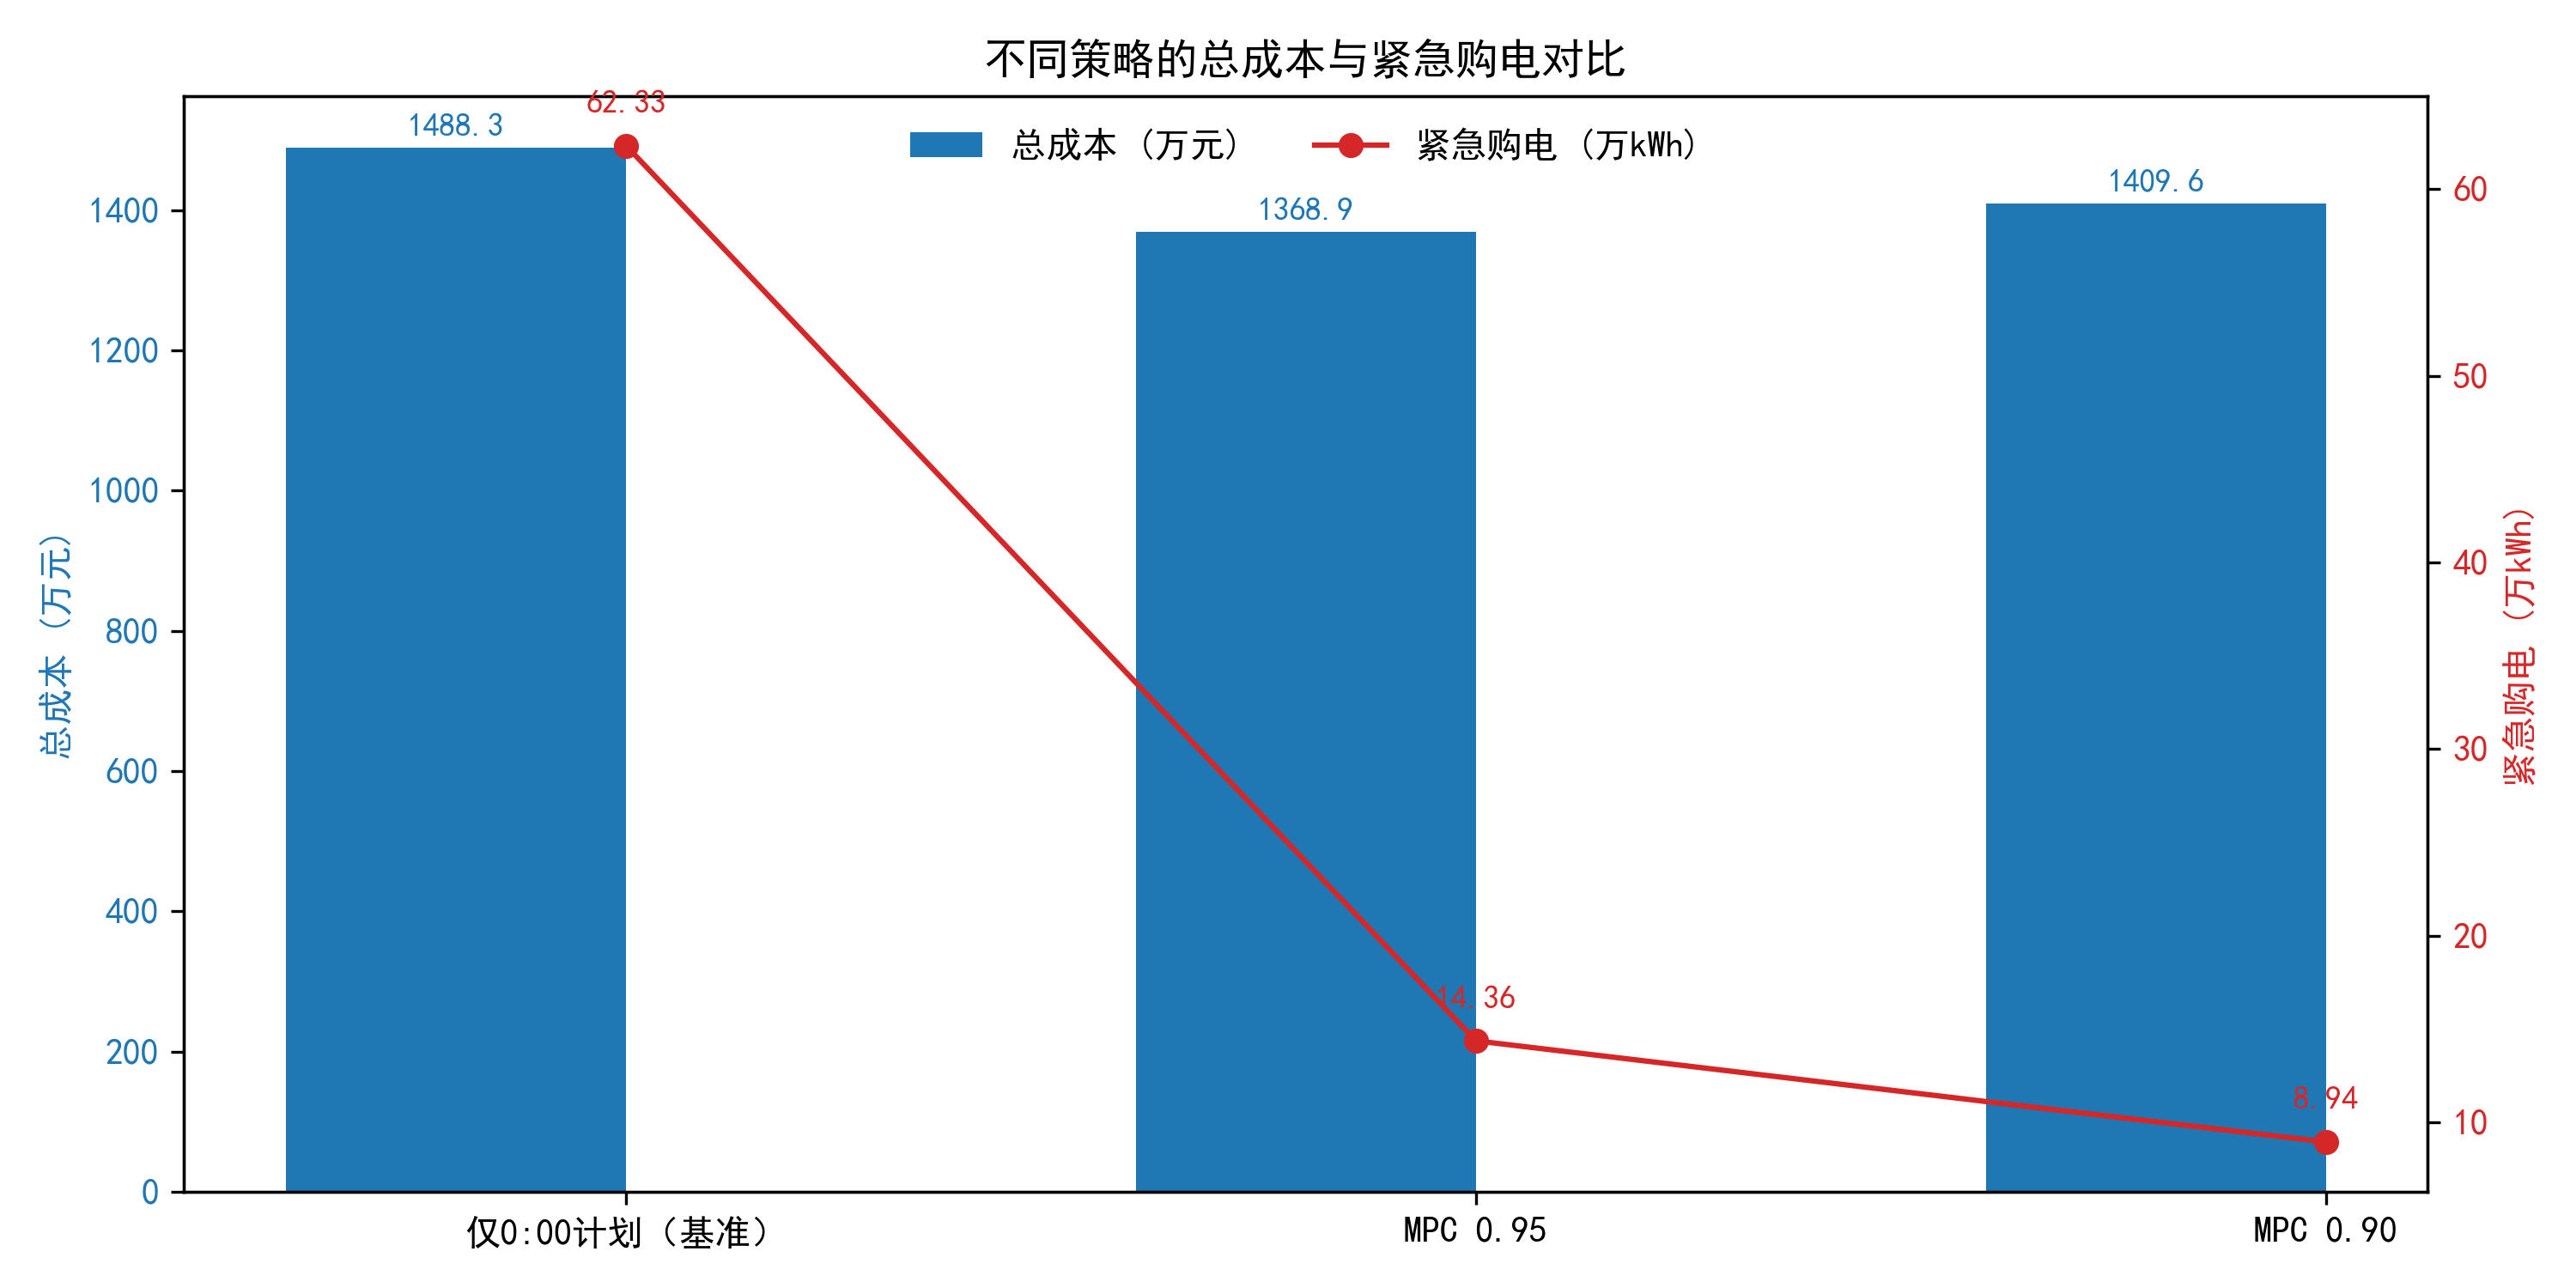
\includegraphics[width=.84\textwidth]{q3_compare.png}
\caption{问题三不同策略的成本与紧急购电对比}
\label{fig:q3compare}
\end{figure}

\begin{figure}[H]
\centering
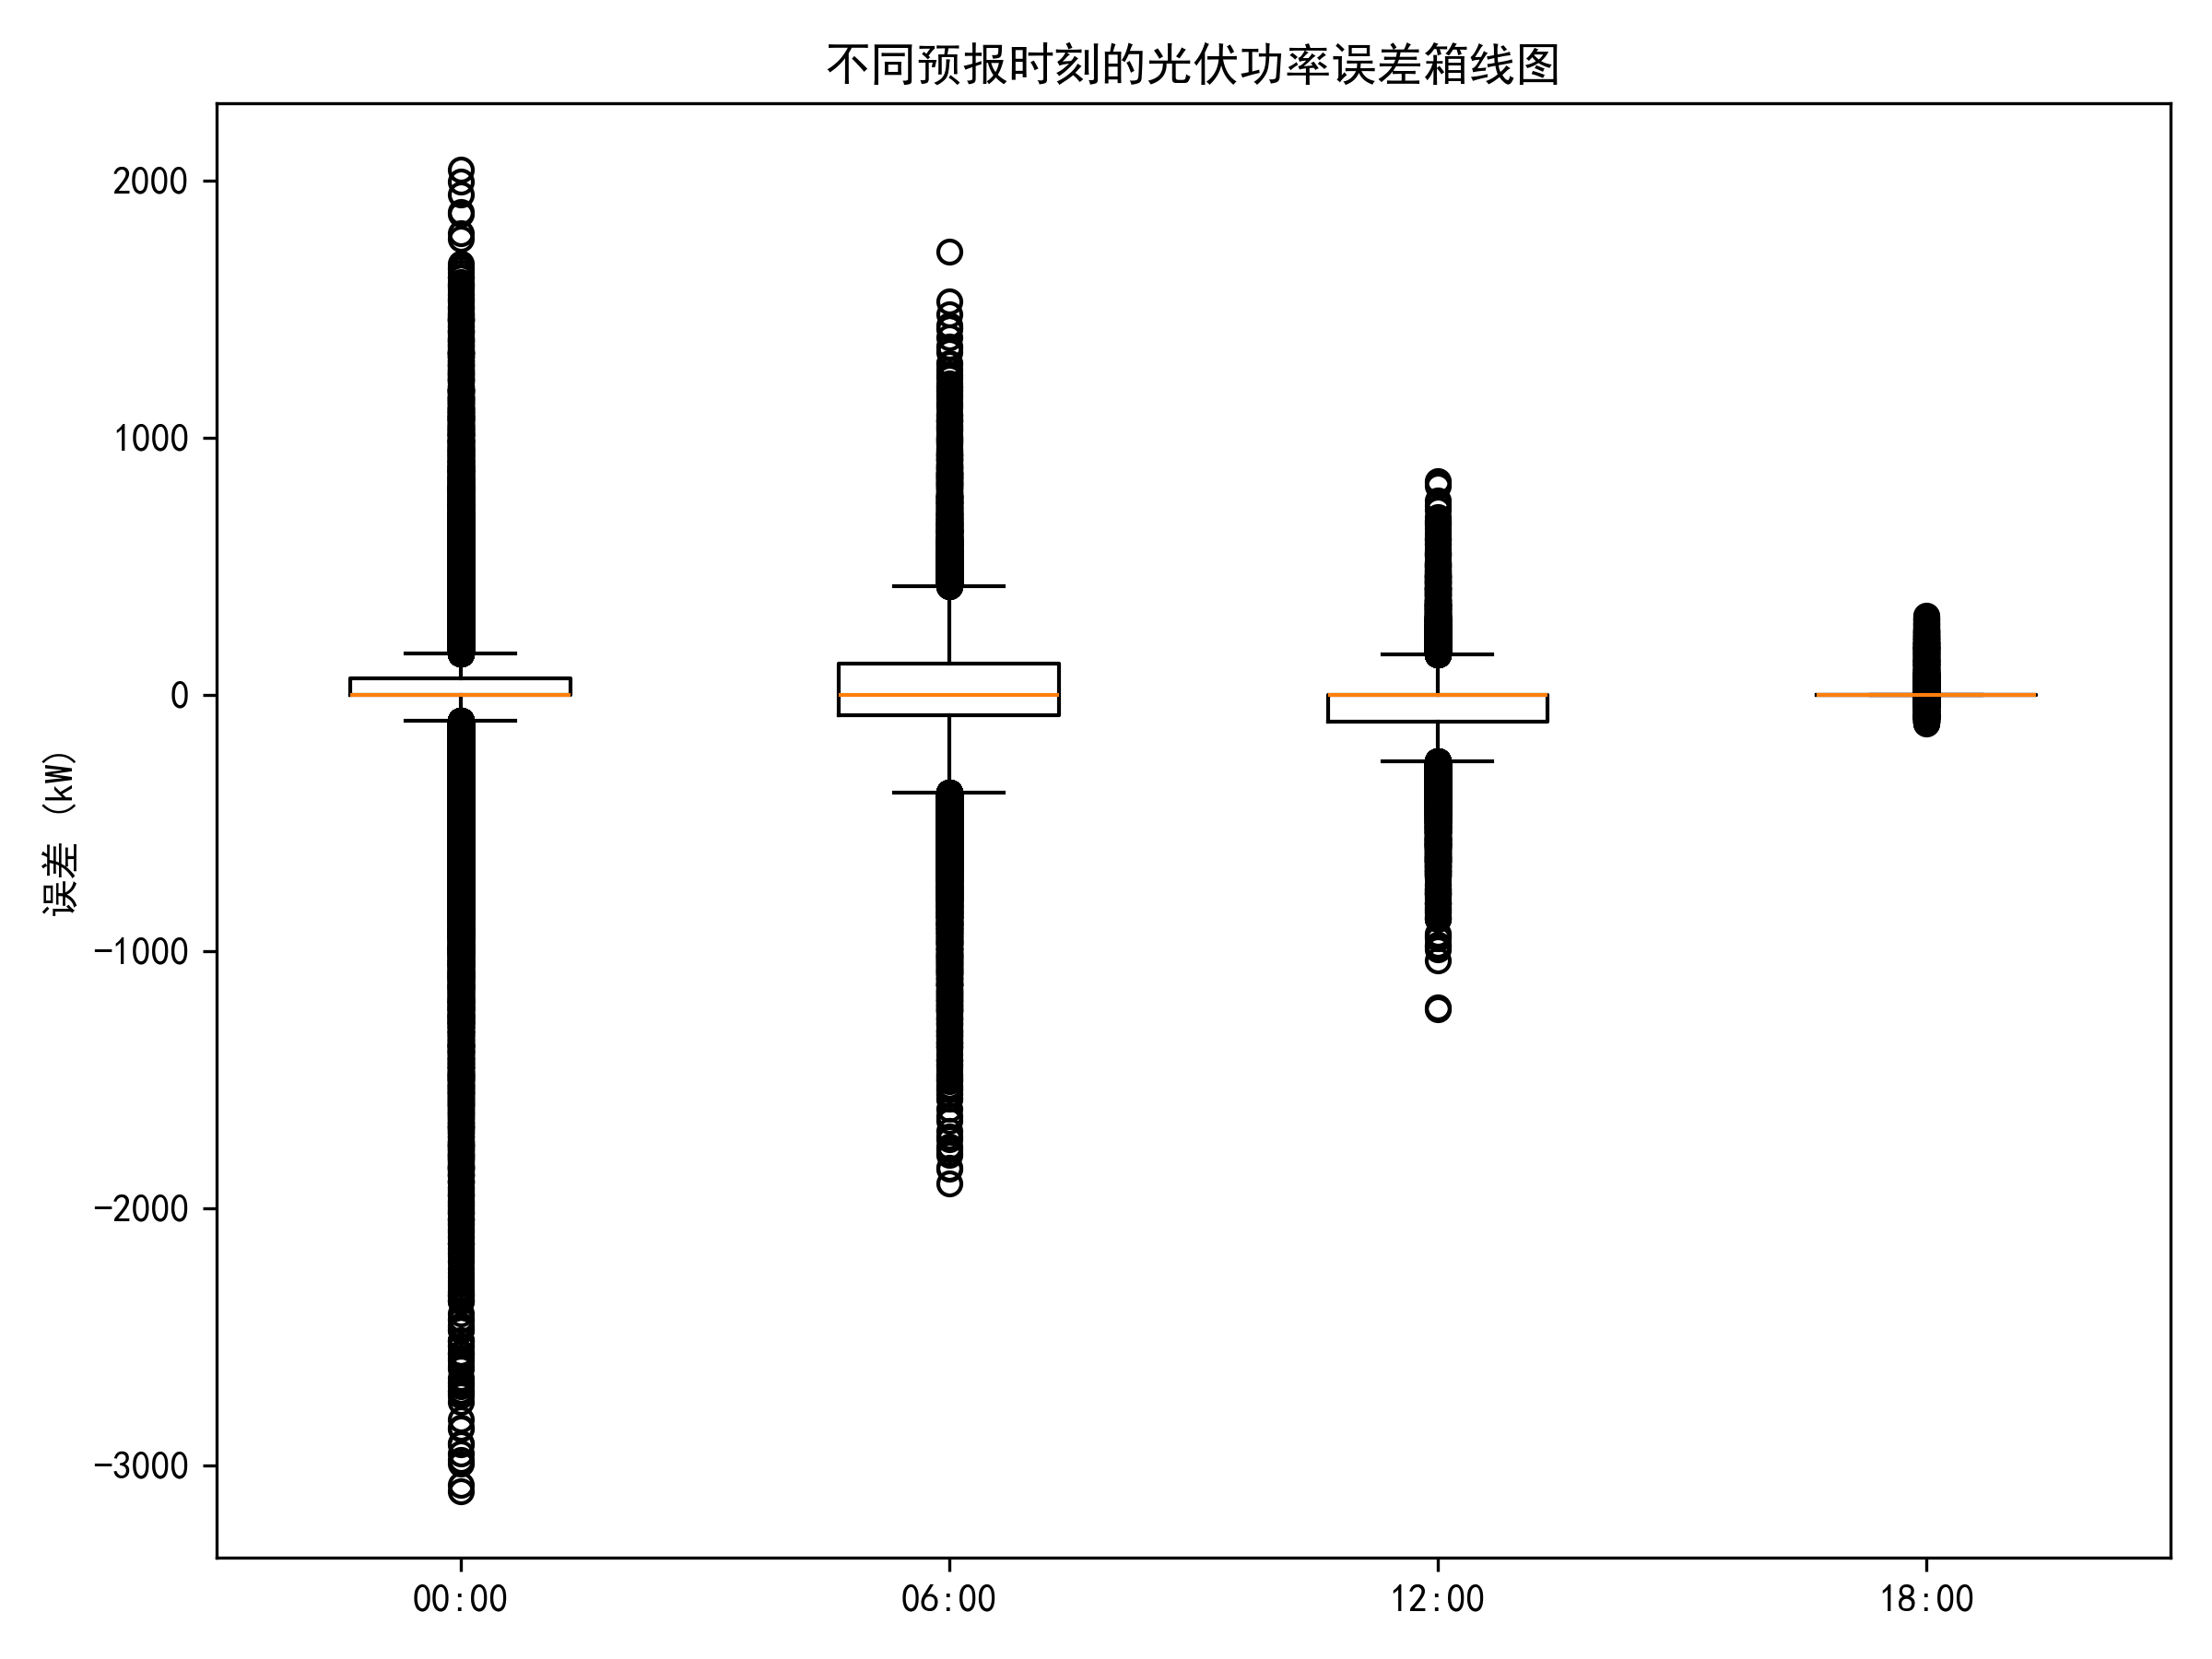
\includegraphics[width=.78\textwidth]{q3_error.png}
\caption{问题三不同发布时间的光伏预测误差}
\label{fig:q3error}
\end{figure}

\begin{figure}[H]
\centering
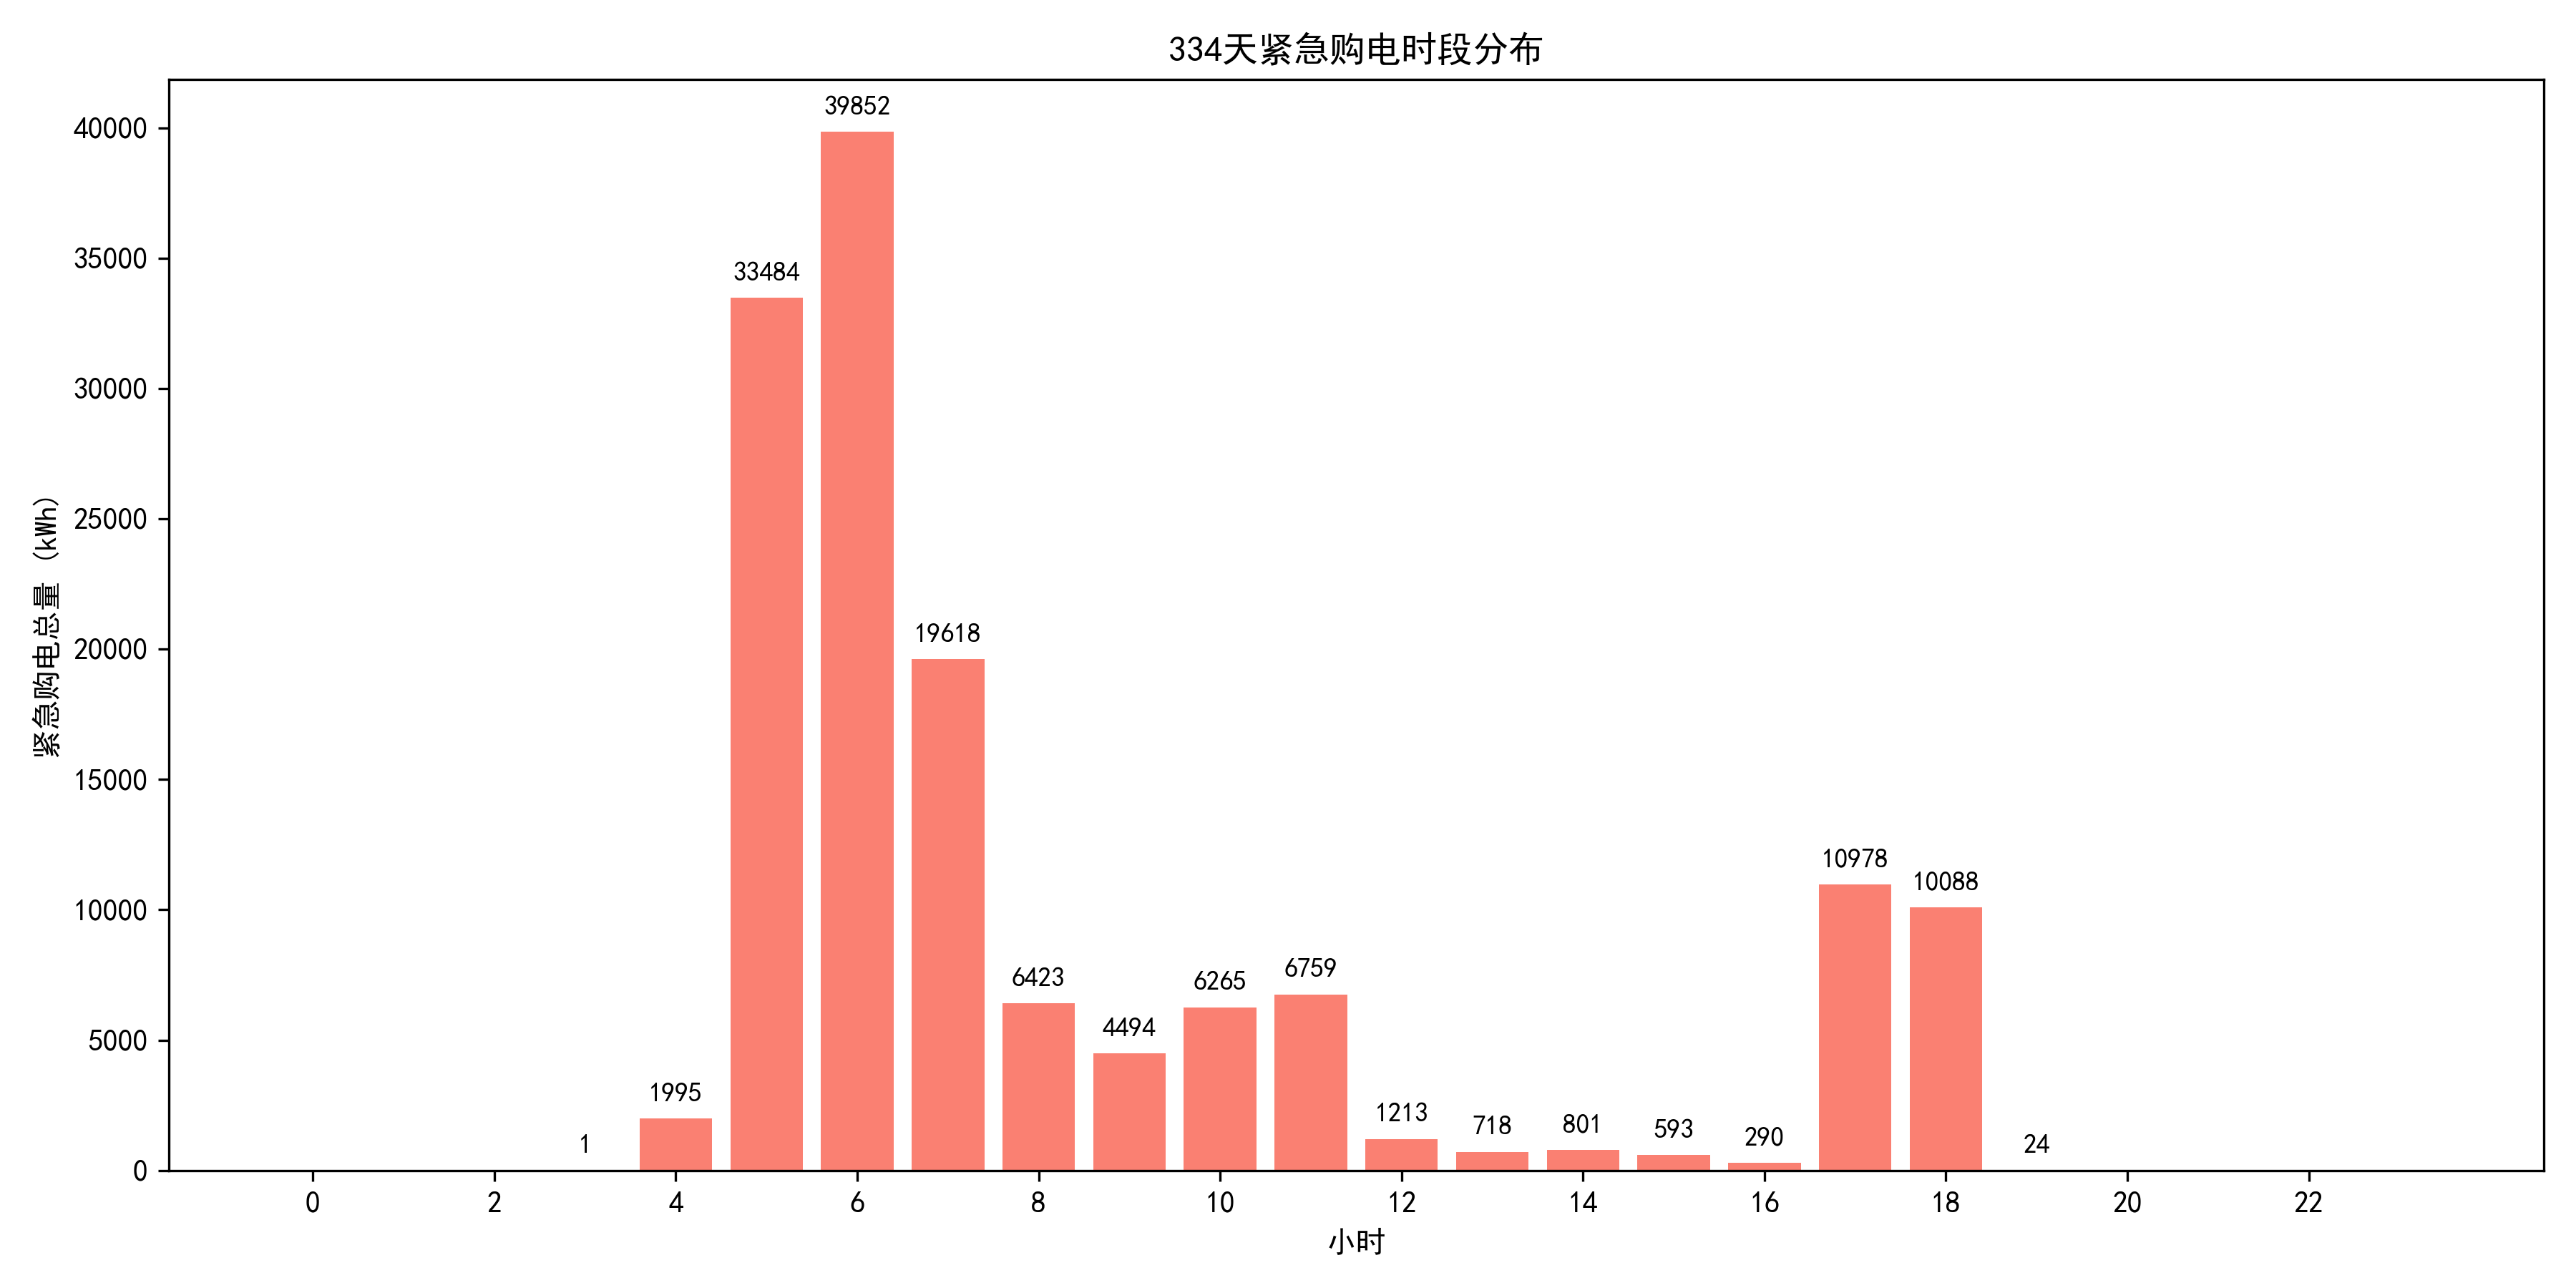
\includegraphics[width=.78\textwidth]{q3_emergency.png}
\caption{问题三紧急购电的小时分布}
\label{fig:q3emergency}
\end{figure}

\section{问题四：动态电价下的机会约束与MPC}

\subsection{动态电价建模}

问题四将基础价格替换为附件4给出的日期--时段动态电价矩阵$C_{d,t}$。日内每一单位购电量的费用随$d,t$变化，因此储能既承担预测误差缓冲作用，又具有低价充电、高价放电的套利动机。对4-2，使用式（10）中的历史净负荷统计量和安全净负荷$\mu_{d,t}+K\sigma_{d,t}$，只需将问题二的目标函数替换为
\begin{equation}
\min Z_{4-2,\mathrm{DA}}=\sum_{t\in\Tset}C_{d,t}E^0_{d,t}.
\tag{24}
\end{equation}
实际结算仍按
\begin{equation}
Z_{4-2}=\sum_{d,t}C_{d,t}E^0_{d,t}+5\sum_{d,t}C_{d,t}E_{\mathrm{emer},d,t}.
\tag{25}
\end{equation}

对4-3，MPC的预测供需平衡使用动态电价下的调整购电量：
\begin{equation}
E_{d,t}+\widetilde E_{\mathrm{pv},d,t}^{(\tau)}+E_{\mathrm{dis},d,t}-E_{\mathrm{ch},d,t}
\geq E_{\mathrm{load},d,t},qquad t\geq\tau,
\tag{26}
\end{equation}
其偏差费用线性化目标为
\begin{equation}
\min Z_{4-3,\tau}=\sum_{t=\tau}^{143}C_{d,t}
\left(E_{d,t}+0.5u^+_{d,t}+0.5u^-_{d,t}\right).
\tag{27}
\end{equation}
真实回测使用附件2的负荷和实际光伏，全天总成本为偏差结算费用与5倍动态电价紧急购电费用之和。动态电价场景取$K=0.80$、$\beta=0.95$；$\beta$用于将日内光伏预测修正为$\widetilde E=\beta\widehat E$。

\subsection{问题四回测结果}

\begin{table}[H]
\centering
\renewcommand\arraystretch{1.2}
\caption{问题四两类动态电价方案对比}
\label{tab:q4main}
\begin{tabular}{lrr}
\toprule
\textbf{指标} & \textbf{4-2} & \textbf{4-3 MPC}\\
\midrule
回测天数 & 334 & 334\\
总成本（万元） & 1740.2419 & \textbf{1433.1927}\\
普通购电或结算成本（万元） & 1578.6095 & 1374.2854\\
紧急购电成本（万元） & 161.6324 & 58.9073\\
紧急购电量（万kWh） & 37.0508 & 14.3723\\
紧急购电天数 & 246 & 334\\
弃光量（万kWh） & 625.1011 & 188.4382\\
\bottomrule
\end{tabular}
\end{table}

4-3的紧急购电量约为4-2的38.79\%，紧急购电成本下降63.55\%，弃光量下降69.86\%。但紧急购电天数由246天增加到334天，说明MPC将少数日期的较大缺口分散为更多日期的小缺口；因此不能只用“发生天数”评价风险。为识别滚动机制的独立作用，在同一4-3信息、价格和结算规则下设置0:00固定计划基准，其总成本为1554.3341万元；MPC总成本为1433.1927万元，节省121.1413万元，节省率7.7938\%。这组对照才是MPC边际收益的主要证据，而4-2与4-3的差异还包含信息结构和模型目标的变化。

\begin{figure}[H]
\centering
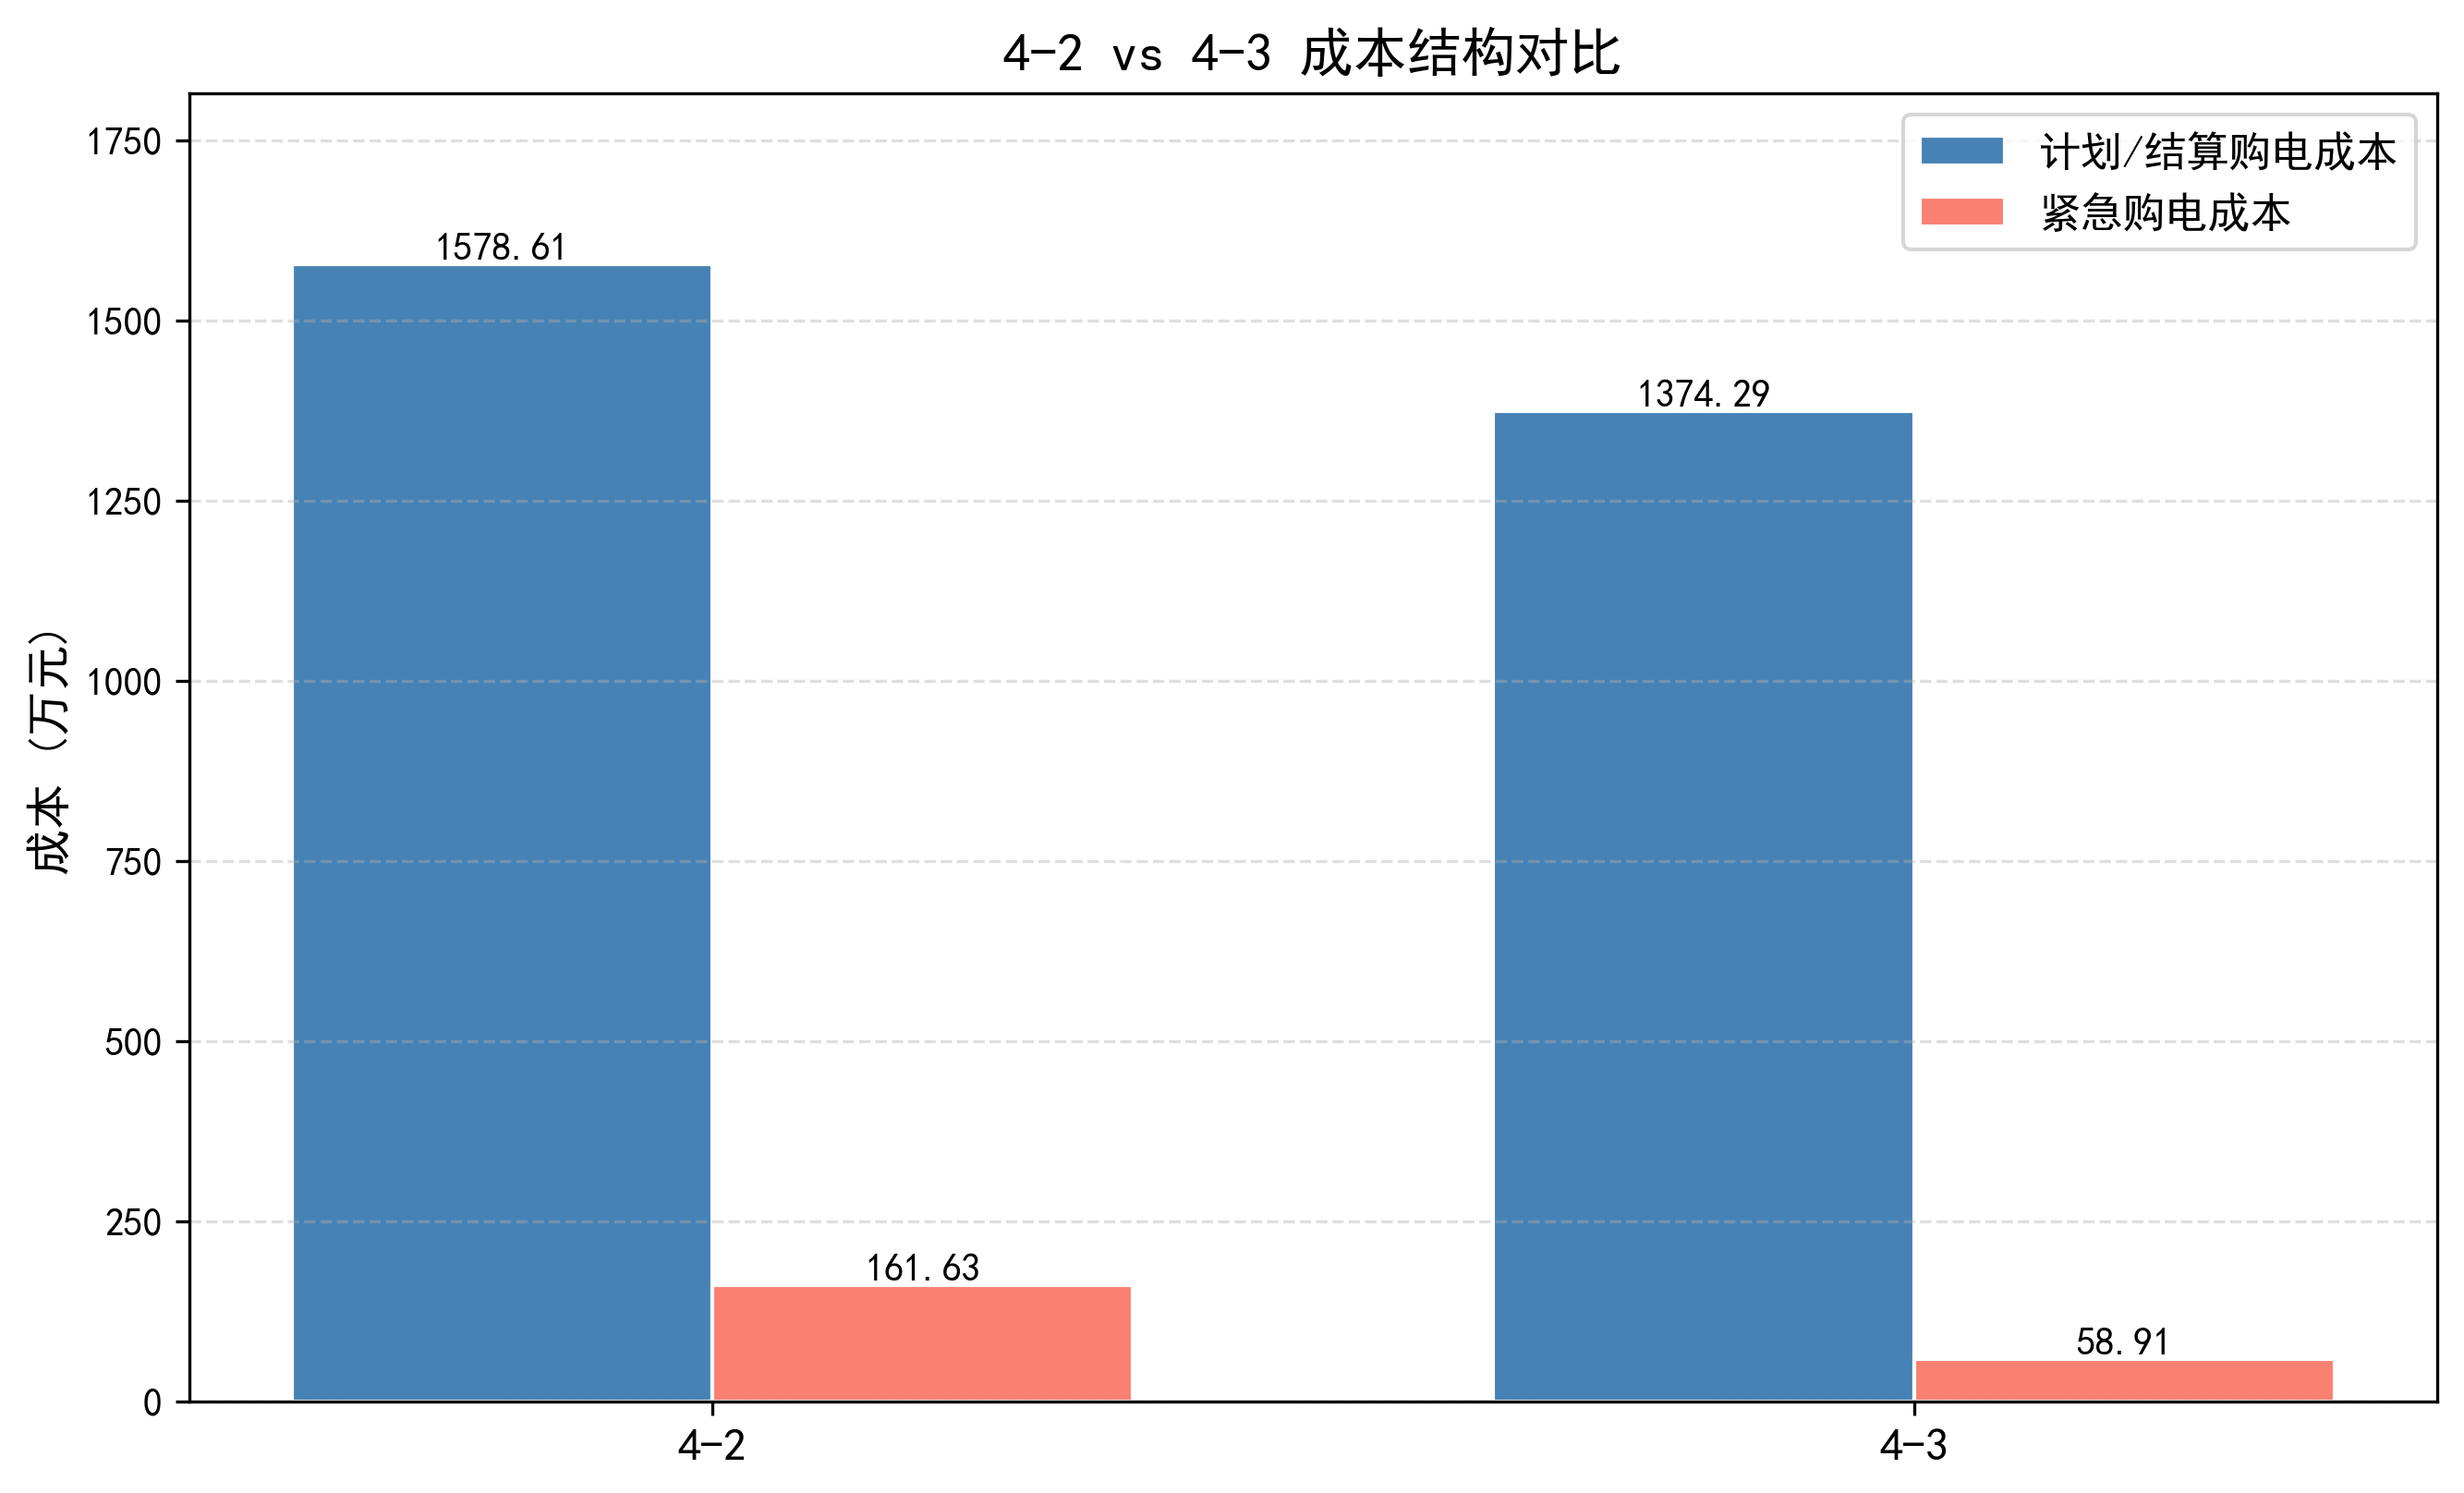
\includegraphics[width=.82\textwidth]{q4_cost.png}
\caption{问题四4-2与4-3的成本结构}
\label{fig:q4cost}
\end{figure}

\subsection{动态电价和参数敏感性}

附件4中日内价差最大的样本日为2025年8月15日，最低电价约0.1119元/kWh，最高电价约1.6114元/kWh。该日调度轨迹呈现低价充电、高价放电，说明动态电价确实进入了储能决策。对$K=0.70,0.75,0.80,0.84,0.90$的4-2敏感性分析显示，$K=0.80$在测试网格上总成本最低；$K=0.84$的紧急购电量更低但总成本略高，可作为可靠性优先的备选。对$\beta=1.00,0.98,0.95,0.90$的4-3敏感性分析显示，$\beta=0.95$取得最低总成本和最高节省率，$\beta=0.90$的紧急购电量更低但保守购电成本上升。

\begin{table}[H]
\centering
\renewcommand\arraystretch{1.2}
\caption{问题四关键参数敏感性摘要}
\label{tab:q4sens}
\begin{tabular}{ccrrr}
\toprule
\textbf{模型} & \textbf{参数} & 总成本（万元） & 紧急购电量（万kWh） & 备注\\
\midrule
4-2 & $K=0.70$ & 1757.7321 & 53.1217 & 风险较高\\
4-2 & $K=0.80$ & \textbf{1740.2419} & 37.0508 & 经济性主方案\\
4-2 & $K=0.90$ & 1746.8967 & 26.0479 & 可靠性优先\\
4-3 & $\beta=1.00$ & 1467.3062 & 34.7520 & 预测不折减\\
4-3 & $\beta=0.95$ & \textbf{1433.1927} & 14.3723 & 主方案\\
4-3 & $\beta=0.90$ & 1476.3934 & 8.9465 & 过度保守\\
\bottomrule
\end{tabular}
\end{table}

\begin{figure}[H]
\centering
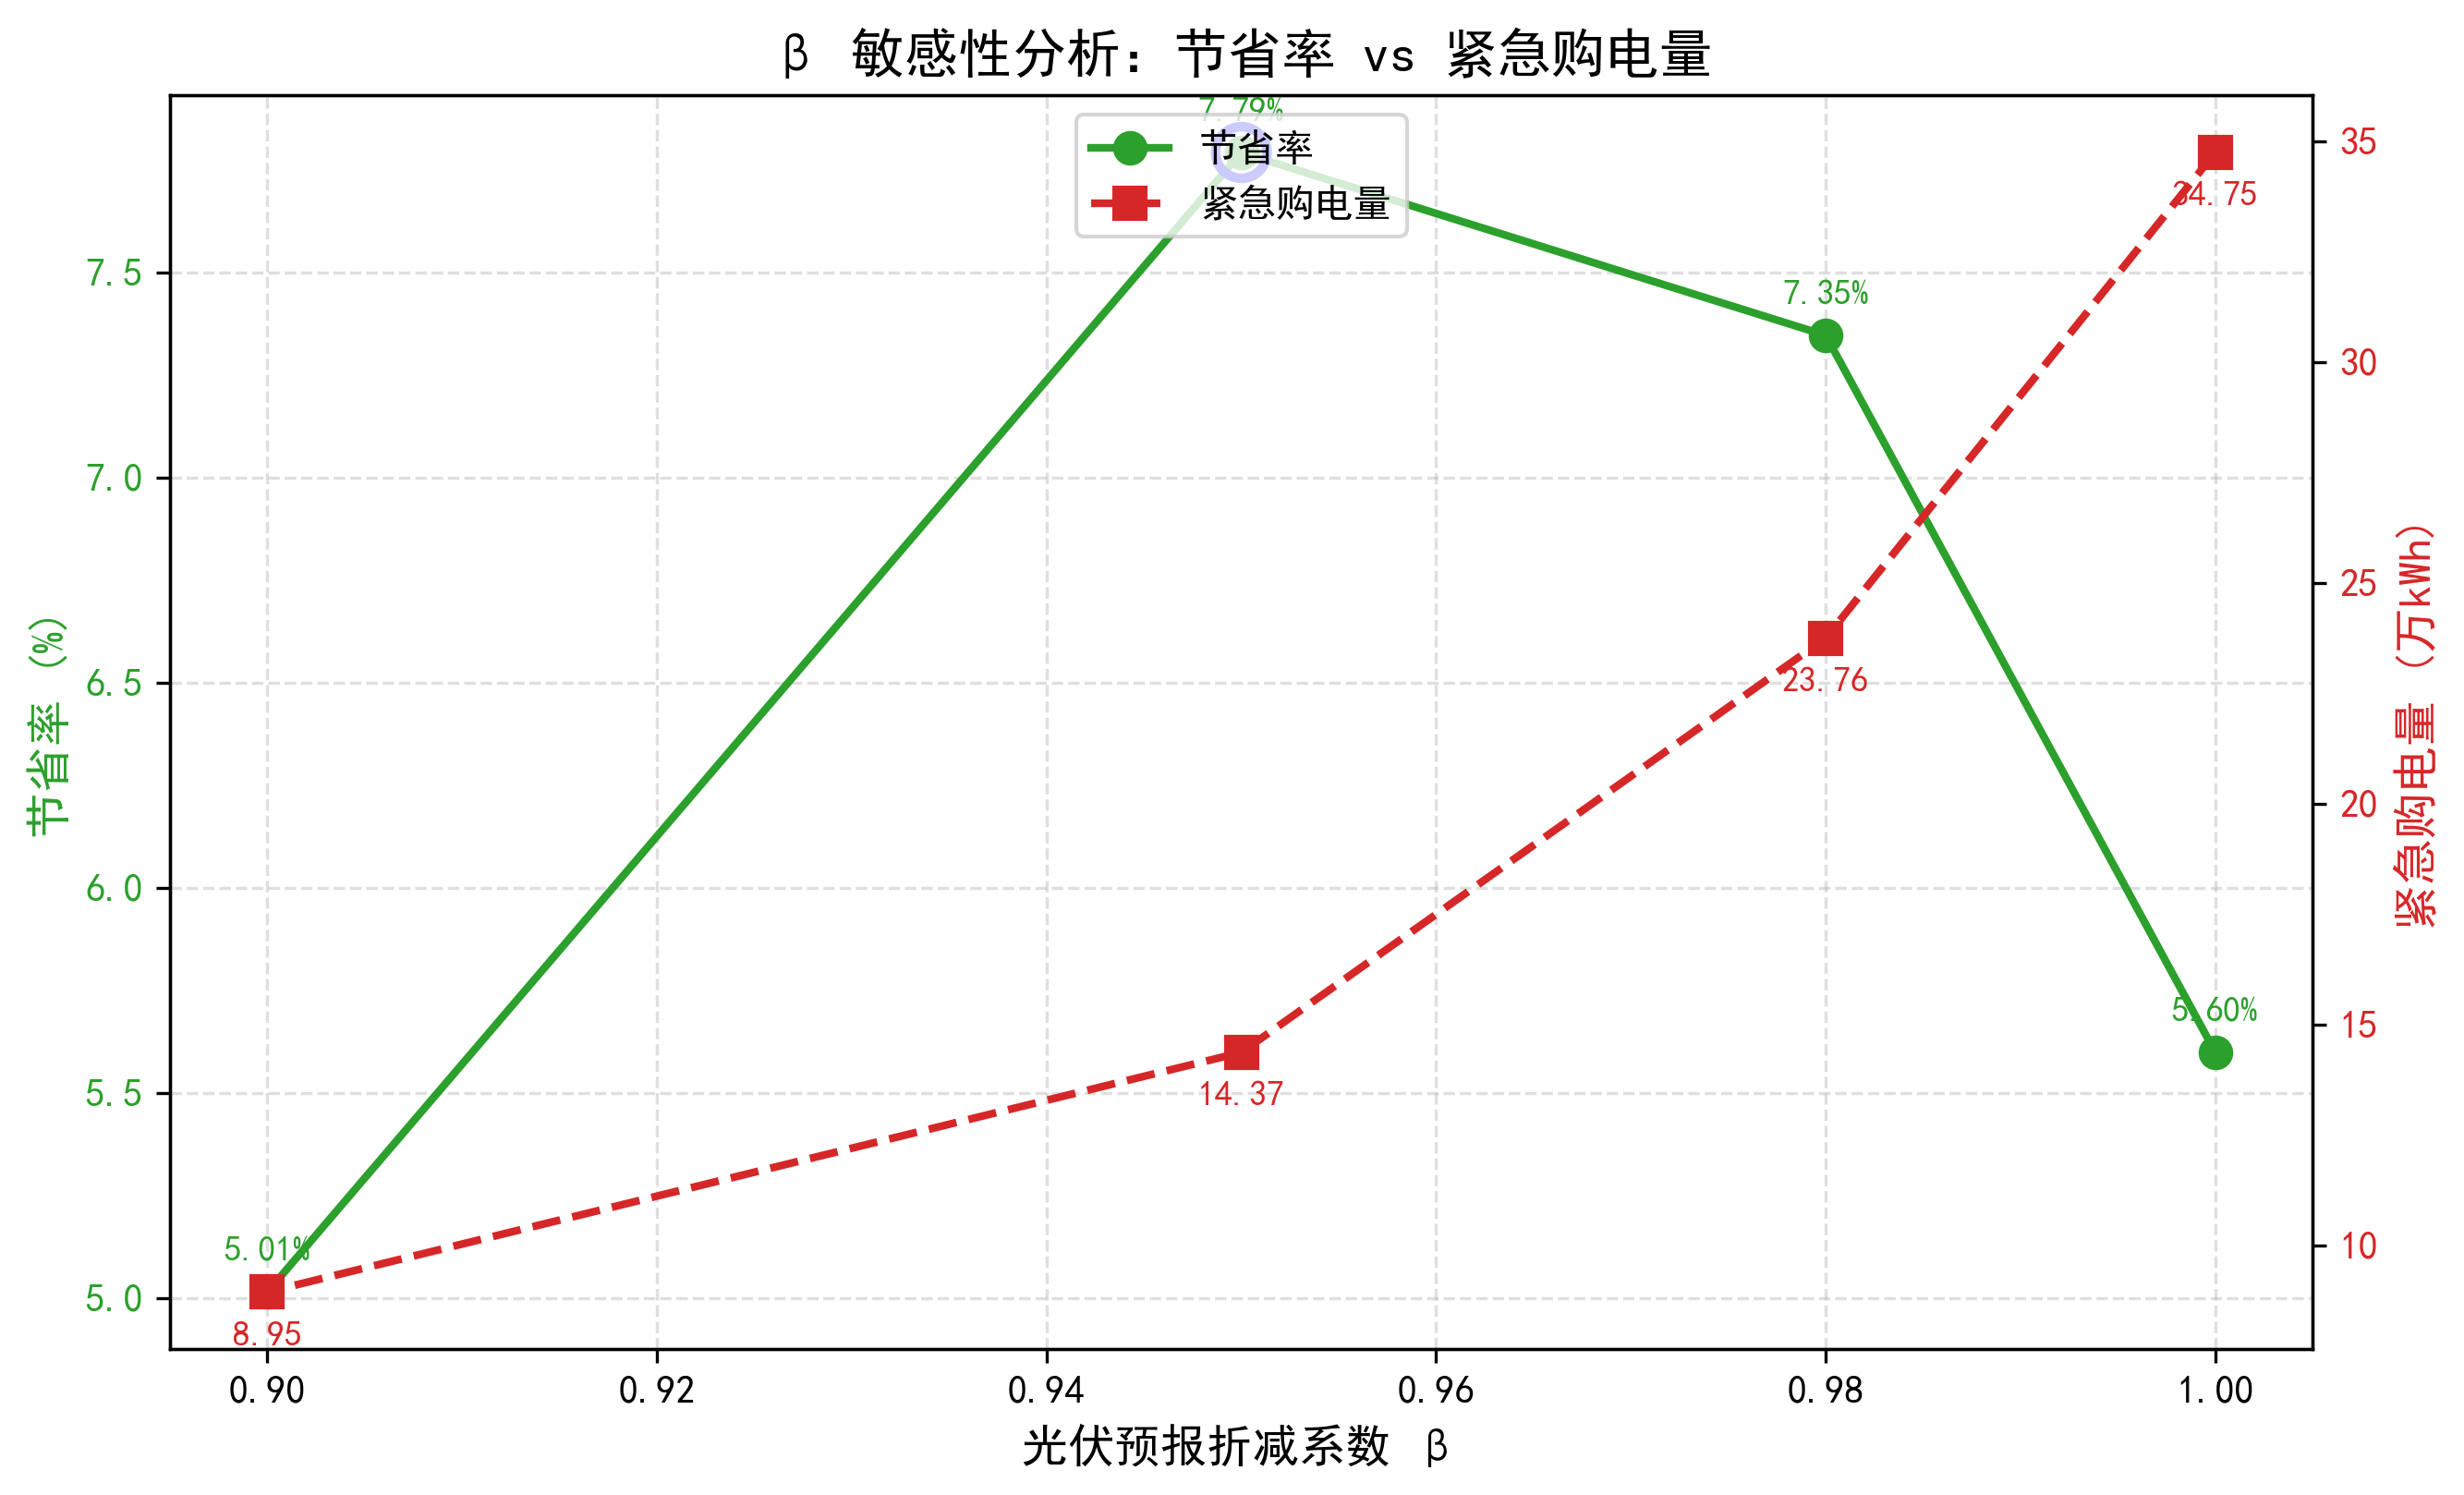
\includegraphics[width=.82\textwidth]{q4_beta.png}
\caption{问题四预测折减系数敏感性}
\label{fig:q4beta}
\end{figure}

\section{统一算法、结果讨论与模型评价}

\subsection{统一求解流程}

四个问题均可在同一线性规划求解框架下实现，差异只在预测信息和电价输入。算法流程如下：
\begin{enumerate}
    \item 将功率数据转换为十分钟电量，按日期匹配附件2至附件4，并检查每一天是否具有144个时段；
    \item 问题一直接使用给定预测；问题二和4-2计算前14天净负荷均值、标准差和安全净负荷；问题三和4-3对四个发布时间的光伏预测进行日期填充、跨日截断、插值和折减；
    \item 在0:00求解全天日前计划；问题三和4-3在6:00、12:00、18:00锁定已执行区间，以真实运行状态为初值重优化剩余时域；
    \item 使用真实负荷和实际光伏进行回测，按储能状态递推计算普通购电、偏差费用、紧急购电和弃光；
    \item 对总成本、紧急购电量、发生天数、弃光量及参数敏感性进行汇总，并按照题目附件5的格式输出结果文件。
\end{enumerate}

由于目标函数和约束均为线性，HiGHS可以对每个日期和每个滚动阶段求得当前信息集下的全局最优解。需要强调的是，滚动优化的“全局最优”是给定预测、状态和费用规则下的单阶段最优，不等同于未知未来真实数据下的全局最优。

\subsection{模型优点}

\begin{enumerate}
    \item 统一采用电量变量，量纲一致，供需平衡和储能状态递推具有直接物理解释；
    \item 将确定性优化、机会约束和MPC逐层衔接，完整描述了从完美预测到不确定预测、再到信息更新的决策演化；
    \item 用增购和退订辅助变量线性化非对称偏差费用，使滚动调整仍可使用线性规划求解；
    \item 通过无储能基准、历史回测、固定计划对照和参数敏感性分析验证经济性与可靠性，避免只报告单一成本；
    \item 明确区分同模型MPC对照与不同模型综合比较，降低了结果解释中的因果混淆。
\end{enumerate}

\subsection{局限与改进方向}

\begin{enumerate}
    \item 本文回测直接使用附件4的动态电价；实际在线运行应使用日前价格预测，并在价格更新后同步滚动优化；
    \item 问题二和4-2的日前目标最小化普通购电费，紧急购电罚费在回测阶段结算，尚未建立含补救变量的完整两阶段随机规划；
    \item 机会约束采用14天历史窗口和正态近似，没有显式刻画负荷误差与光伏误差的联合分布；可改用场景随机规划、分布鲁棒优化或联合机会约束；
    \item $\alpha$和$\beta$由有限历史样本网格选择，没有独立测试集，结论属于样本内比较；
    \item 每日设置始末储电量均为6000\kwh，便于题目要求下的逐日比较，但没有模拟全年连续SOC传递；实际部署时应把上一日终点作为下一日初值。
\end{enumerate}

\section{结论}

本文将C题四个问题统一为微网购电与储能调度的递进式优化体系。问题一的确定性线性规划证明了储能可以利用价格差异和光伏富余降低购电费用；问题二通过历史净负荷的机会约束将预测不确定性转化为可调安全裕度；问题三利用0:00、6:00、12:00和18:00的光伏预测更新，通过MPC滚动修正计划；问题四则将日期--时段动态电价纳入日前和日内目标，使储能同时承担风险缓冲和峰谷套利。

在题目数据和日循环边界下，问题一单日费用下降26.90\%；问题二固定$K=0.80$的334天总成本为1654.76万元；问题三$\alpha=0.95$的MPC总成本为1368.87万元，相对静态计划节省8.03\%；问题四动态电价下4-2和4-3总成本分别为1740.24万元和1433.19万元，4-3相对同模型固定计划节省7.79\%。因此，滚动预测更新在本样本上能够降低综合成本和紧急购电量，但可靠性与经济性仍由安全裕度、预测折减和储能边界共同决定。

上述结论仅适用于本文采用的历史样本、参数网格、费用口径和逐日闭环假设。若要用于真实微网调度，应进一步加入价格预测、跨日SOC传递、负荷预测误差、光伏误差场景和独立测试期，并重新标定风险参数。

\end{document}
